\documentclass{article}
\usepackage[utf8]{inputenc}
\usepackage{attachfile2}
\usepackage{hyperref}
\usepackage{booktabs}
\usepackage{graphicx}
\usepackage{subcaption}
\usepackage{float}
\usepackage{amssymb}
\usepackage{amsfonts}
\usepackage{amsmath}
\usepackage{bookmark}
\usepackage{listings}
\lstset{
  basicstyle=\ttfamily\small,
  numbers=left, 
  numberstyle=\tiny,
  frame=single,
  captionpos=b
}

\raggedbottom

\title{
  Finding the communities inside a graph about political blogs \\
  \vspace{0.5cm}
  \large Network Analysis - Assignment 1}

\author{Enrico Pezzano}

\date{June 2025}

\begin{document}

\maketitle

\section{Introduction}\label{sec:intro}
In this report, I will analyze a graph about political blogs, which is a hyperlink graph of US political blogs collected in early 2005. 
Each node corresponds to an individual blog, and each directed edge ($u \rightarrow v$) indicates that blog $u$ contains at least one hyperlink to blog $v$. The dataset is available at \url{http://konect.cc/networks/political-blogs/}, it captures the "blogosphere" of the time in the 2004 U.S.A. presidential election, and it has become a standard benchmark for community detection algorithms and polarization studies in networks and social media analysis.

In the following sections, I will list the main characteristics and properties of the chosen graph, analyze its communities and evaluate their quality, and finally, I will show them in different colors by drawing the graph.


\section{Part 1: Graph characteristics}\label{sec:part1}
After having introduced the graph and its domain, I will compute its key properties using the NetworkX Python library. Note that the graph is directed, but I will consider the undirected version for some properties, because many global metrics -such as the diameter, the average clustering coefficient, and the Louvain label vector- are not defined for directed graphs.
I will also attach the resultant output of the code both in the appendix and in assignment archive as a text file.

Starting from the size, the graph has $n = 1224$ nodes and $m = 33430$ edges. The average degree is $\langle k \rangle = 54.6$, which indicates that each blog links to approximately 55 others on average, reflecting moderate connectivity within the network. 
Its maximum degree is $k_{\max} = 702$ and the minimum degree is $k_{\min} = 2$. 

\paragraph{Density and scaling analysis}
I first computed the exact density with the \texttt{nx.density} function, which is defined as
\[
\rho \;=\;\frac{2m}{n(n-1)}
\;=\;
\frac{2\cdot 33430}{1224\,(1224-1)}
\;\approx\;0.0223,
\]
so that means that only about $2.23\%$ of all possible links are present. This number alone already tells that the graph is intuitively \textbf{sparse}, as expected from a hyperlink political graph. But I wanted a more mathematical way to determine that, so I also performed a scaling analysis of the number of edges $m$ as a function of the number of nodes $n$. In other words I wanted to check if the number of edges grows linearly (or not) with the number of nodes, which would indicate that if the graph is really dense or sparse, as seen during lectures and in the slides in the following definitions.

\begin{itemize}
  \item if $\rho \to$ \textbf{costant} when $N\to\infty$, then the graph is \textbf{dense} and $m=O(n^2)$.
  \item if $\rho \to$ \textbf{0} when $N\to\infty$, then the graph is \textbf{sparse} and $m=O(n)$.
\end{itemize}

To do that, I computed the growth exponent $\alpha$ of the number of edges $m$ as a function of the number of nodes $n$, i.e.\ $m\sim n^\alpha$.  If $\alpha\approx1$, then $m=O(n)$ and the graph is sparse; if $\alpha\approx2$, then $m=O(n^2)$ and the graph is dense. In short, $\rho$ measures the \textbf{current} density of the graph, and $\alpha$ measures the "tomorrow's" density, i.e.\ how $m$ will grow as $n$ increases: in practice, I am checking if the links between nodes grow as fast as the number of nodes.

To estimate $\alpha$, I used the following formula.
\[
\alpha \;\approx\;\frac{\ln m}{\ln n}
\;=\;
\frac{\ln(33430)}{\ln(1224)}
\;\approx\;1.46.
\]
Because $\alpha$ lies much closer to~1 than to~2, we have $m=O(n)$ rather than $O(n^2)$ and hence $\rho\to0$ in the large-$n$ limit.  In other words, the network is rigorously \emph{sparse}. 

Another way to check if the graph is sparse is the compare $m$ with the minimum number and the maximum number of edges in a directed graph with $n$ nodes, i.e.\ $m_{\min}=n-1$ and $m_{\max}=n(n-1)$.  In this case, we have $m_{\min} = 1223$ and $m_{\max} = 1496952$, and we can see that $m$ is much closer to $m_{\min}$ than to $m_{\max}$, which confirms again that the graph is sparse.

The following listing shows the relative python code that I used for what I just described.
\begin{lstlisting}[language=Python, label=fig:code-density]
density = nx.density(G)
print(f"Density: {density:.4f}")

alpha = np.log(m) / np.log(n)
print(f"Scaling exponent alpha = {alpha:.3f}")

if abs(alpha - 2) < abs(alpha - 1):
  print("G is DENSE")
  print("m grows around O(n^2), so alpha->const")
else:
  print("G is SPARSE")
  print("m grows around O(n), so alpha->0.")
\end{lstlisting}

\vspace{0.5cm}

Since the graph is not globally connected, I computed the finite diameter on its largest connected component, obtaining $d_{\max} = 8$.

The following code snippet, instead, shows how I computed the characteristics mentioned above.
\begin{lstlisting}[language=Python, label=fig:code-part1]
print("Number of nodes:", G.number_of_nodes())
print("Number of edges:", G.number_of_edges())
avg_degree = np.mean([d for n, d in G.degree()])
print("Average degree:", avg_degree)
print("Max degree:", max(dict(G.degree()).values()))
print("Min degree:", min(dict(G.degree()).values()))

all_lengths = nx.all_pairs_shortest_path_length(G)
max_dist = 0
for source, dist_dict in all_lengths:
    # dist_dict only contains reachable targets
    local_max = max(dist_dict.values(), default=0)
    if local_max > max_dist:
        max_dist = local_max
print("Finite reachability diameter:", max_dist)
\end{lstlisting}

\subsection{Connected Components}
\label{sec:components}
As already mentioned, the $polblogs$ graph is not completely globally connected, so I computed the number of connected components and their respective sizes. The resultant output showed that there are 2 connected components, with sizes $1222$ and $2$, this means that the graph would have been completely connected if it was not for those two remaining nodes, which are isolated from the rest of the graph and connected by themselves. 
The following code snippet shows the function that I implemented in order to obtain the previous mentioned results.
\begin{lstlisting}[language=Python, label=fig:code-CCs]
wccs = list(nx.weakly_connected_components(G))
sccs = list(nx.strongly_connected_components(G))

if len(wccs) == 1:
  print("Graph is weakly connected")
else:
  largest_wcc = max(wccs, key=len)
  print(f"G is not connected ({len(wccs)} components); "
      f"largest WCC size = {len(largest_wcc)}")
  G_lcc = G.subgraph(largest_wcc)
  print("\tLargest WCC strongly connected? ",
      nx.is_strongly_connected(G_lcc))

if len(sccs) == 1:
    print("G is strongly connected")
else:
  print(f"G is not a SCC ({len(sccs)} components); "
  f"largest SCC size = {len(max(sccs, key=len))}")

print("\nComponent size summary:")
print(f"\t# WCCs: {len(wccs)}")
print(f"\tWCC sizes: {sorted(map(len, wccs))}")
print(f"\t# SCCs: {len(sccs)}")
print(f"\tSCC sizes: {sorted(map(len, sccs))}")
\end{lstlisting}

Obviously, the 2 strongly connected components are the same ones of the weakly connected components, i.e.\ every SCC (by definition) is also a WCC, but not vice versa.
In other words, that means that there are 2 political blogs disconnected to the rest of the network, but still connected to each other (forming a SCC), and that the largest component ($1222$ nodes) is strongly connected.

This observed behaviour is a typical situation in political blogs networks, where some blogs are not linked to the main network, but still have a few links between them, forming isolated communities, i.e.\ bubbles.

\subsection{Average Clustering Coefficient}
The \emph{average clustering coefficient} $\bar C$ of a graph on $N$ nodes is defined as
\[
\bar C \;=\;\frac{1}{N}\sum_{i=1}^N C_i,
\]
where each local coefficient
\[
C_i = \frac{2L_i}{k_i(k_i-1)}
\]
measures the fraction of “closed” triplets (triangles) in the neighborhood of node~$i$.

\paragraph{Domain.} 
By construction,
\[
0 \;\le\; C_i \;\le\;1
\quad\Longrightarrow\quad
0 \;\le\;\bar C\;\le\;1.
\]

For this graph we obtain
\[
\bar C \approx 0.32,
\]
and at a first glance I assumed this value was synonym of a low clustering coefficient, but then I compared it against a random graph built with the configuration model function of \texttt{NetworkX} which returned a clustering coefficient of \(C_{\mathrm{rand}} \approx 0.25\).
After that, I confirmed that the \texttt{polblogs} graph has a higher clustering coefficient -since \(C_{\mathrm{obs}} > C_{\mathrm{random}}\)-, meaning that the political blogs network is more clustered than a random graph with the same number of nodes and edges.
This indicates a higher number of local-clustering blogs that tend to link within cohesive groups rather than uniformly at random, forming a higher number of structural holes.
In practice, the result is the formation of some clusters of blogs that are more densely connected to each other than to the rest of the network, which is typical in political blog networks where parties or ideological groups tend to link to each other more frequently than to blogs outside their sphere, forming tightly knit groups.
The following code snippet shows how I computed the values above.

\begin{lstlisting}[language=Python]
avg_cc = nx.average_clustering(G.to_undirected())
print(f"Avg clustering coefficient: {avg_cc:.4f}")

deg_seq = [d for _, d in G.degree()]
R = nx.configuration_model(deg_seq, 
          create_using=nx.Graph())  
R.remove_edges_from(nx.selfloop_edges(R))

rand_C = nx.average_clustering(R)
print(f"Random baseline clustering: {rand_C:.4f}")

if avg_clustering > rand_C:
  print("Clustering is higher than baseline")
else:
  print("Clustering is not higher than baseline")
\end{lstlisting}

\subsection{Assortativity - "birds of a feather flock together"}
The assortativity coefficient for the $polblogs$ graph is \(r = -0.2212\). 
This negative number means that nodes with high degrees tend to connect to nodes with lower degrees, which makes for a disassortative mixing pattern. 
The graph will probably create "star-like" hubs of highly connected blogs. This is common in political blog networks, where big blogs may link to smaller, less popular ones instead of forming dense clusters with other hubs, e.g. The New York Times links to smaller political blogs instead of other big news papers.
I used the right NetworkX function on the original directed graph to find the assortativity coefficient.

%  Does the graph have the same characteristics of a random or a power-law network?

\subsection{Comparison with Random and Power-Law Models}
\label{sec:model-comparison}
To assess whether the political-blogs network behaves more like an Erdős–Rényi random graph or a scale-free (power-law) network, I could already that the graph is more similar to a power-law network, but I wanted to be more precise, so I had to compare key empirical statistics against the expectations of these two canonical models. In the following, I will summarize the main findings already discussed in the previous subsections.

\paragraph{Graph characteristics.}
\[
  C_{\mathrm{obs}} \approx 0.32,\quad
  \rho \approx 0.0223,\quad
  r \approx -0.2212.
\]

As described in the previous section and confirmed by the above values, the \texttt{polblogs} graph has a high clustering coefficient, low density, and negative assortativity.
Each of these features is a signature of a power-law network, as confirmed graphically by the degree distribution plot in the following figure, which shows the resultant degree distribution of the political blogs network, compared to a Barabasi–Albert model with the same number of nodes and edges. 

\begin{figure}[H]
  \centering
  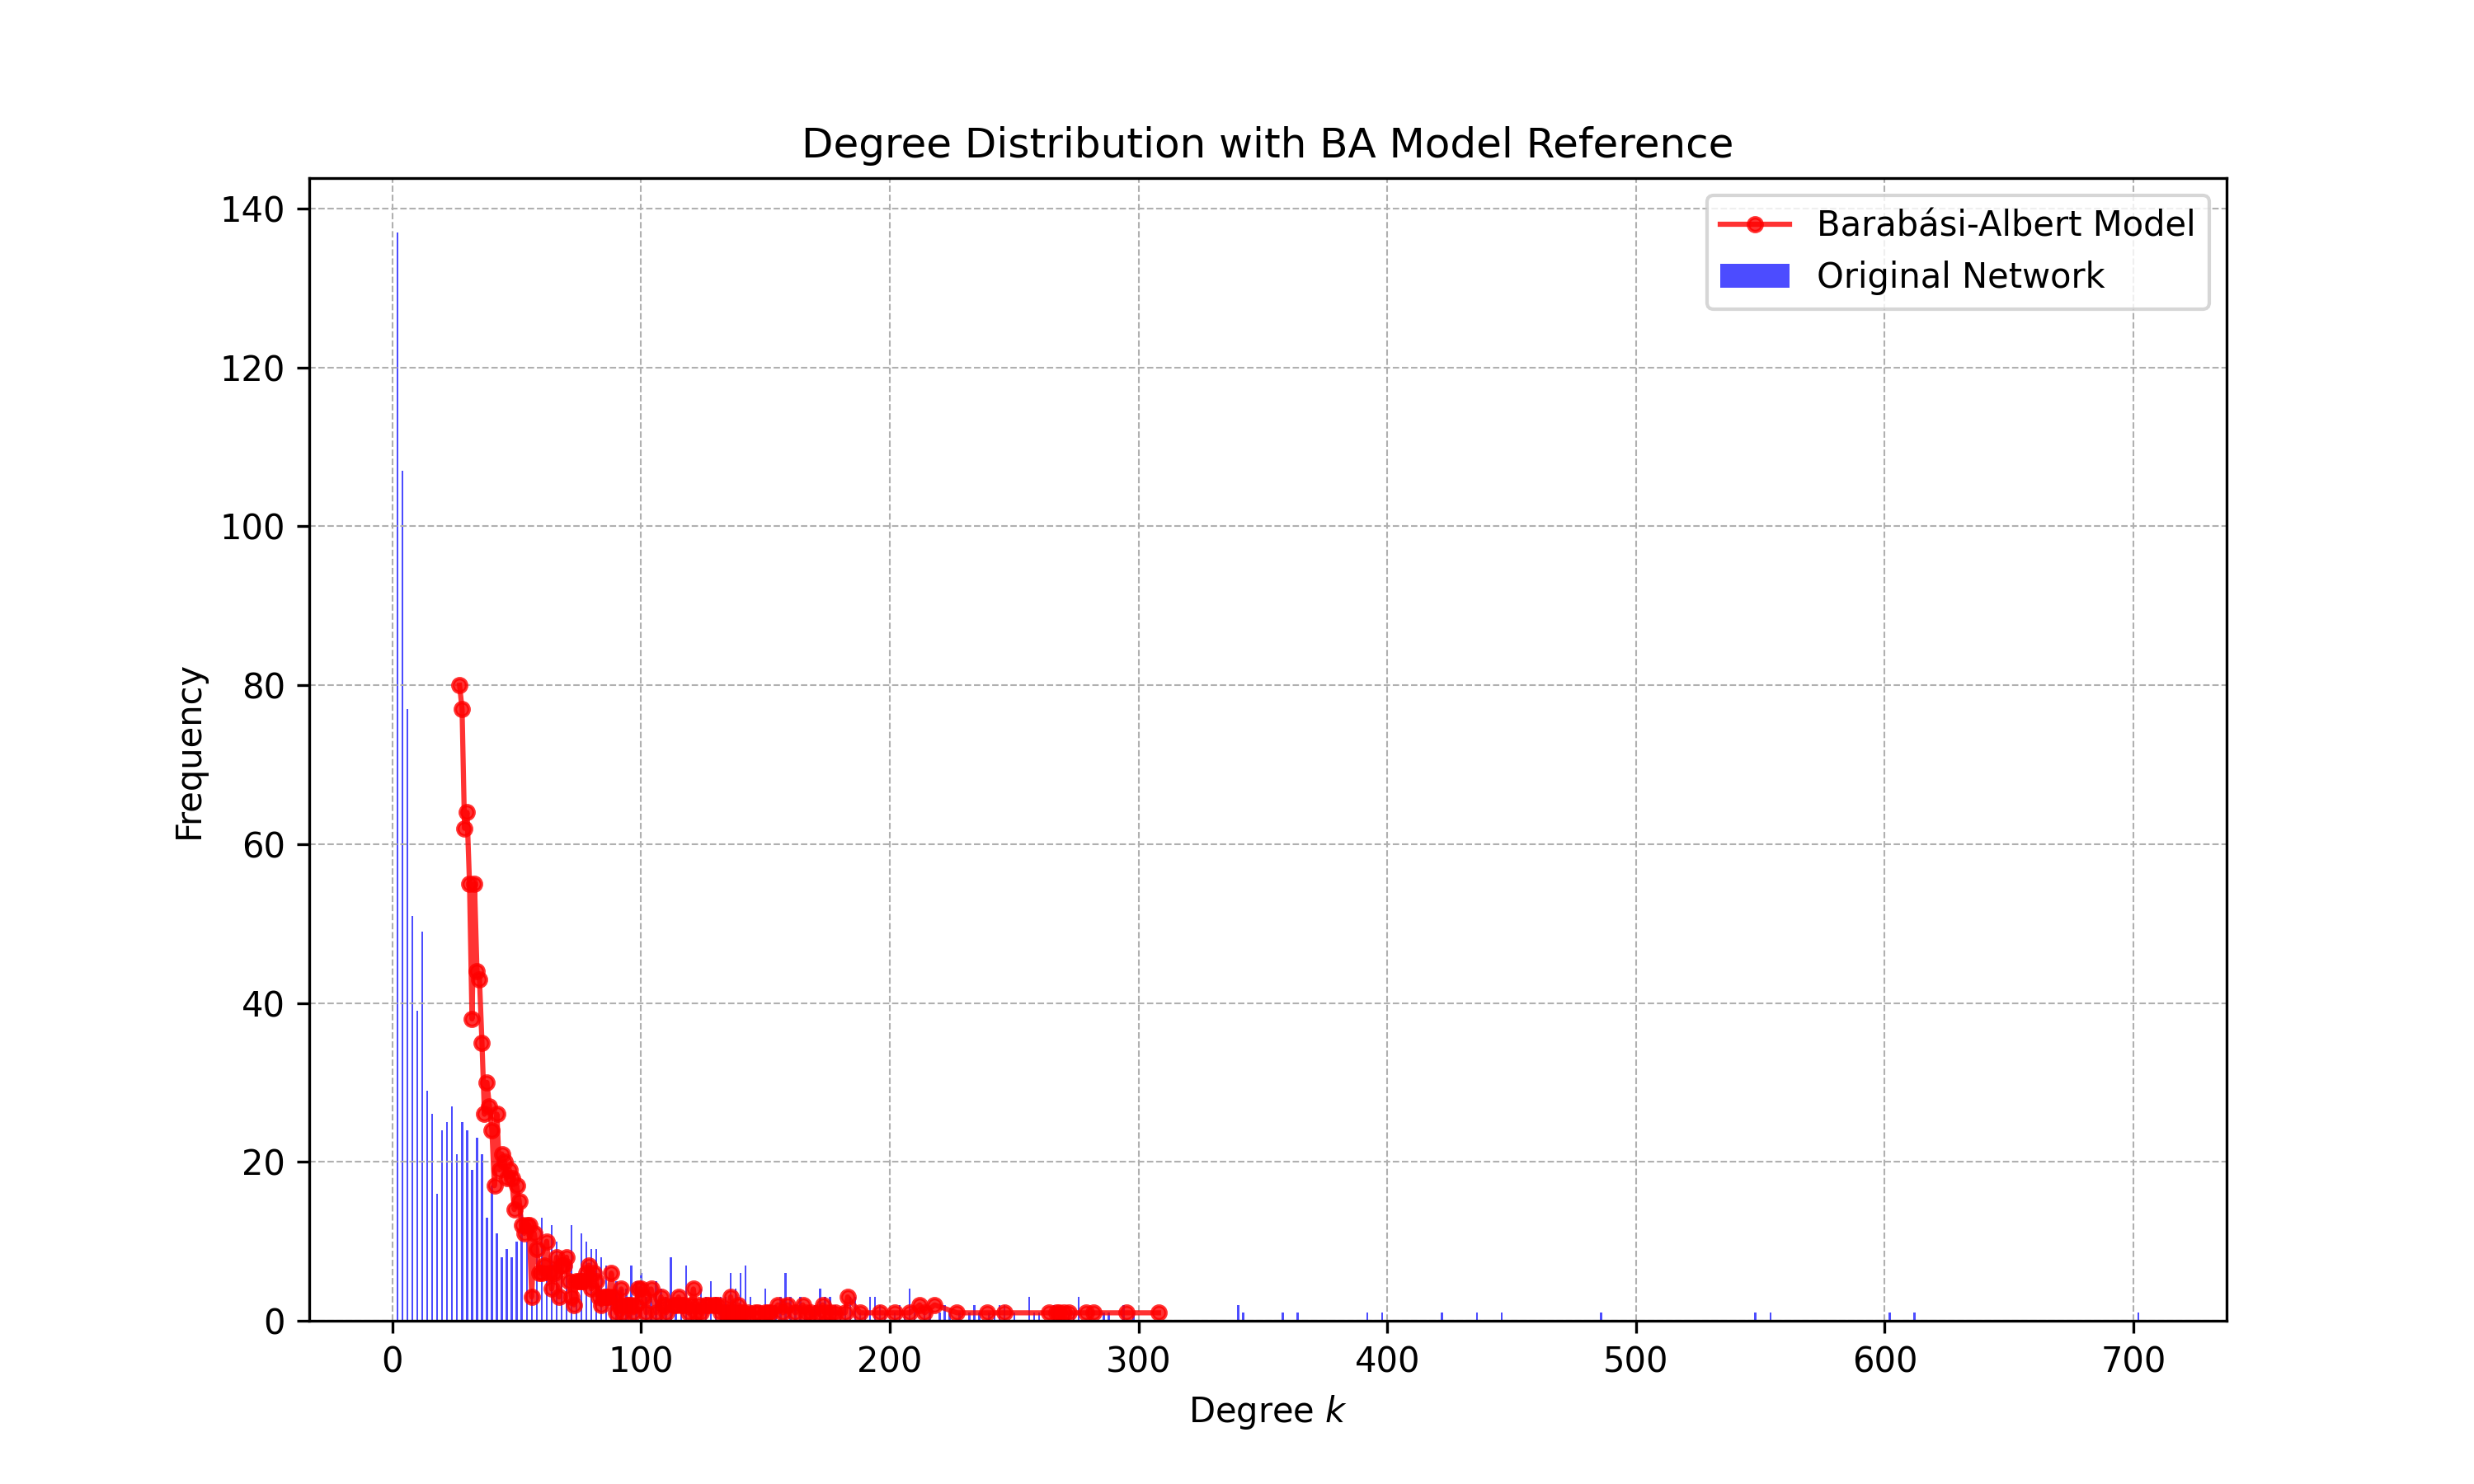
\includegraphics[width=1\textwidth]{../images/degree_distribution.png}
  \caption{Vanilla degree distribution of the political blogs network.}
  \label{fig:degree-dist}
\end{figure}


\paragraph{Small-world characteristics.}
Despite being a sparse graph, the political blogs network combines:
\begin{itemize}
  \item \emph{High clustering} (\(C_{\mathrm{obs}}=0.32\)).
  \item \emph{Average shortest-path length} (\(\bar{\ell}_{\mathrm{obs}}=2.74\))
\end{itemize}

Even though the average shortest-path length is more than the theoretical average shortest-path for an equal size random graph, i.e. \ $t = \log(n)/\log(k) = 1.78 < 2.74 = \bar{\ell}_{\mathrm{obs}}$, it is still safe to assume the $2.74$ is a very low value for a graph with $n=1222$ nodes, and significantly shorter than the expected average path length in a random graph, where \(\bar{\ell}_{\mathrm{ER}} \sim n^{1/2}\approx 35.0\).
Note that, in order to compute the average shortest-path length, it is necessary to use the largest connected component, since the graph is not globally connected.
The following code snippet shows how I computed the average shortest-path length; in particular, this time I chose to obtain the subgraph by removing the connected component of size $2$ (since the information gathered before showed that they were the only disconnected nodes), instead of passing the largest connected component to the function.

\begin{lstlisting}[language=Python]
Gsub = G.copy()
sccs = list(nx.strongly_connected_components(Gsub))
for scc in sccs:
  if len(scc) == 2:
    Gsub.remove_nodes_from(scc)
    break
    
try:        
  avg_path_length = nx.average_shortest_path_length(Gsub)
  print(f"Avg shortest path length: {avg_path_length:.2f}")
  t = np.log(n) / np.log(k)
  print(f"Theoretical avg s. p. for random graph: {t:.2f}")
except nx.NetworkXError as e:
    print(f"Error calculating average path length: {e}")
\end{lstlisting}

\vspace{0.5cm}

Finally, I can conclude that this political blogs network exhibits also some small world characteristics, despite its sparsity, it combines a relatively high clustering coefficient with very a very average short path ($2.74$), enabling efficient communication across the entire blogosphere, even if the short path are probably inside the same community, as we will see in the next sections.


% Degree distribution (include a plot)
\subsection{Degree Distribution}
In addition to the "vanilla" degree distribution plot shown above, I also generated a log-binned histogram to better visualize the distribution of degrees across the nodes.
Again, I used a Barabasi–Albert reference model to compare the two distributions.

\begin{figure}[H]
  \centering
  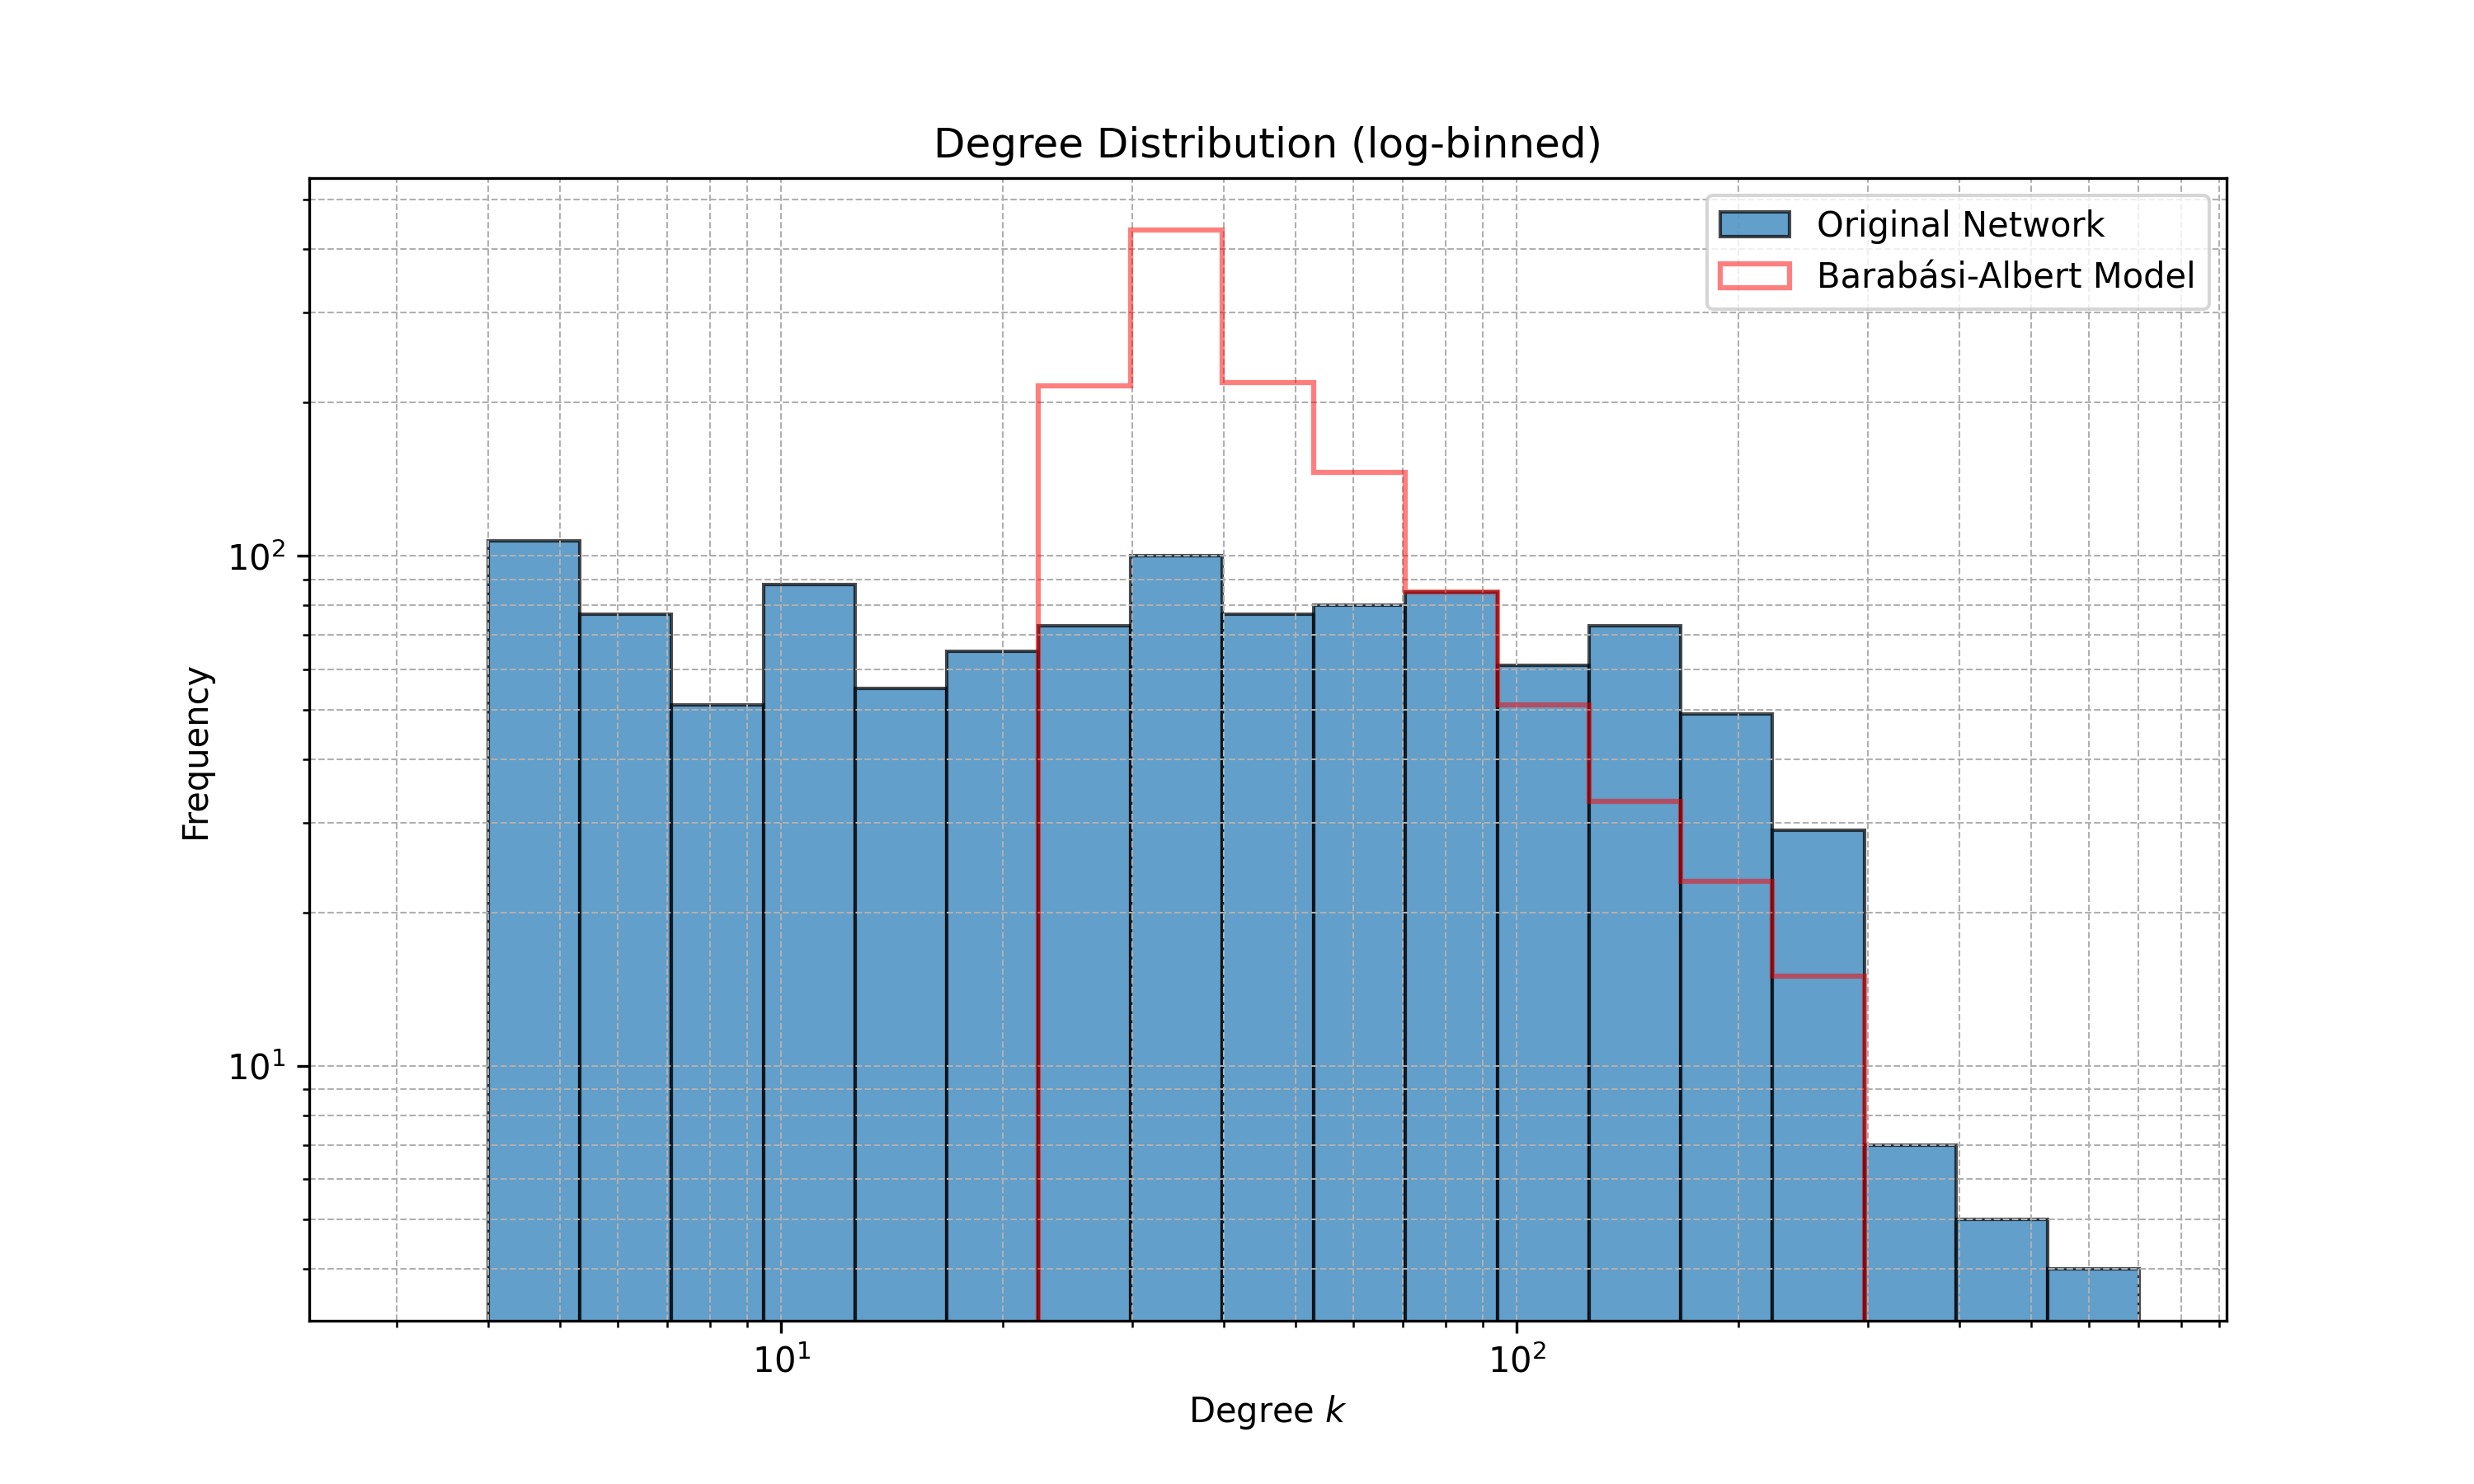
\includegraphics[width=1\textwidth]{../images/degree_distribution_logbinned.png}
  \caption{\label{fig:degree-hist}Degree distribution of the political blogs network}
\end{figure}

Although not clear as in the previous figure, also in this log\-binned histogram, we can see that the degree distribution is not completely equal to the Barabasi–Albert model, but it is still very similar to it, with a few high-degree hubs and many low-degree nodes. 

\subsection{Additional Plots}
\label{sec:additional-plots}
Other than the log-binned histogram, I also implemented the generation of three more plots, in order to explore more the graph.

First, the complementary cumulative distribution (CCDF) of node degree is plotted in the following figure.
\begin{figure}[H]
  \centering
  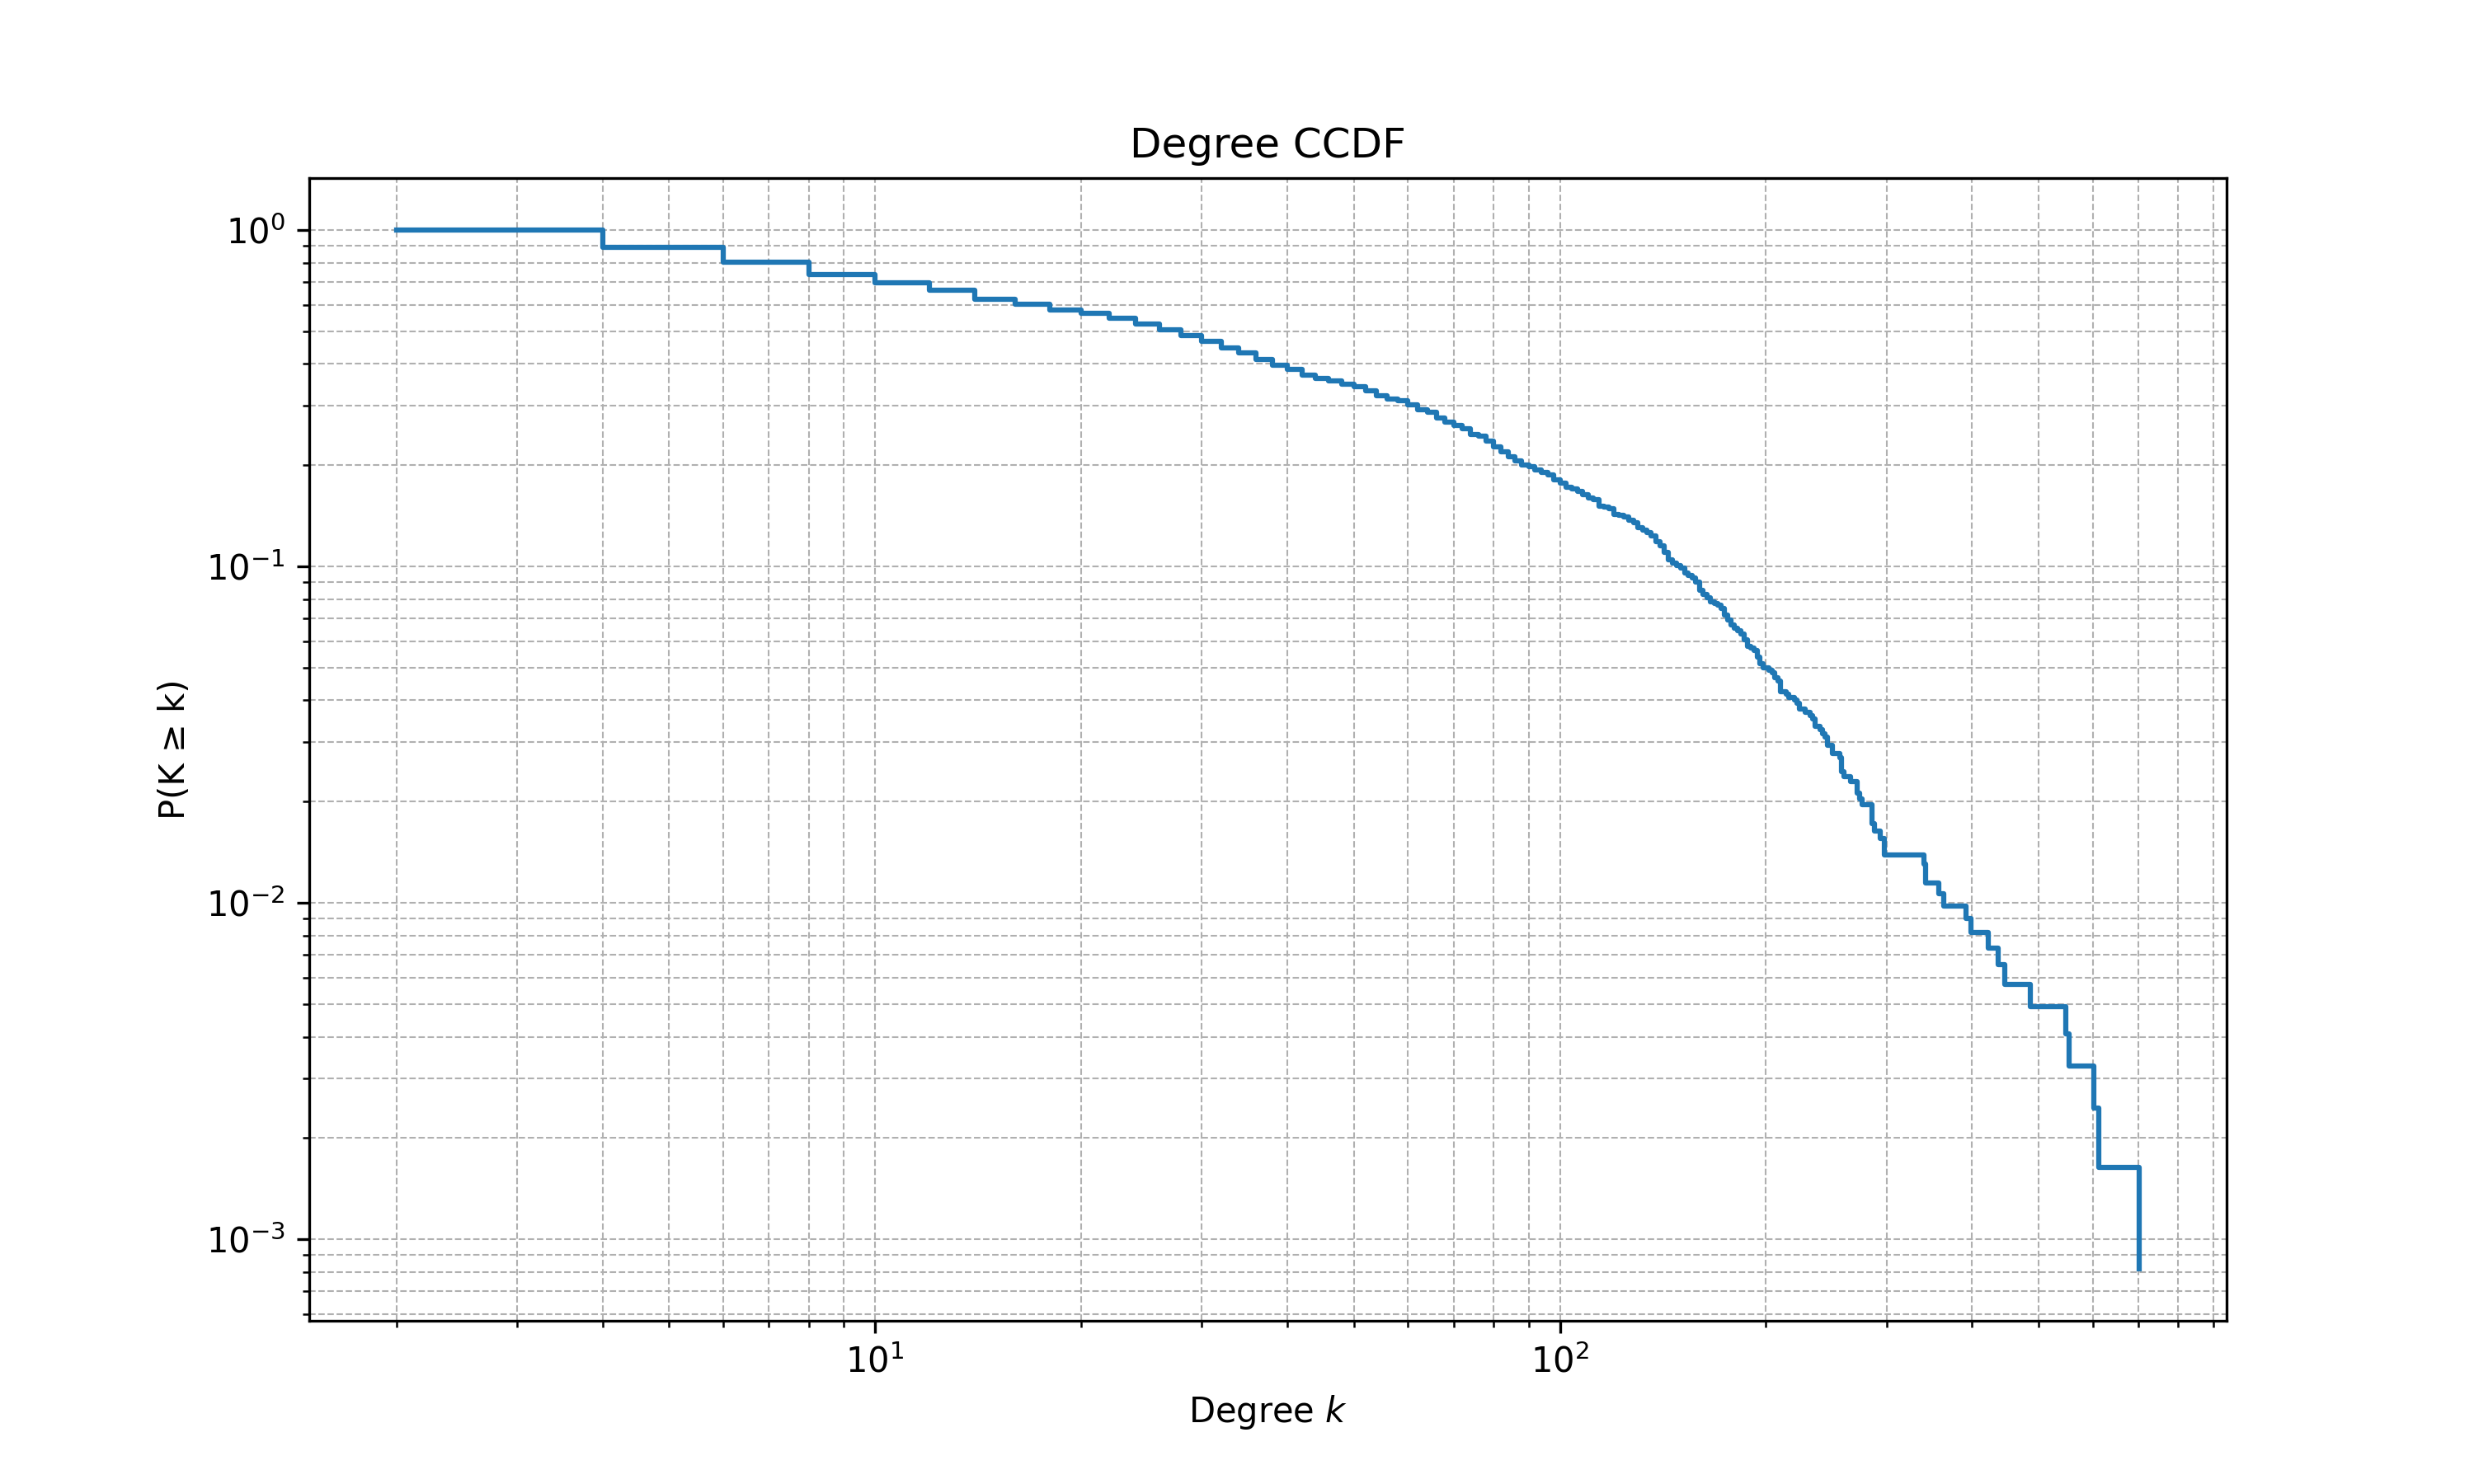
\includegraphics[width=1\textwidth]{../images/degree_ccdf.png}
  \caption{Degree CCDF: \(P(K \ge k)\) on log–log axes.}
  \label{fig:degree-ccdf}
\end{figure} 


This curve is plotted on logarithmic axes and makes the "tail" of the degree distribution very clear. We can read off, for example, that every node has degree at least 2 (the curve starts at 1.0 when $k=2$), that about half the nodes have degree $\geq 8$, and that only a few percent have degree $\geq 100$. 
The roughly straight line decline in the middle range ($10 \lesssim k \lesssim 100$) again points to a heavy tailed (near power law) regime, that means that there is no single "typical" degree, but rather many low degree nodes and a few very high degree hubs. At very large $k$ (above a few hundred), the curve steepens and dips below $10^{-2}$ or even $10^{-3}$, reflecting the finite size of the political blogs network: only a handful of blogs have hundreds of links.

This is an additional confirmation that while most blogs link only to a few dozen others, a small fraction serve as highly connected hubs—an archetypal signature of a sparse, small world, heavy tailed network.


Next, a scatter plot of the raw \((k,\text{count})\) pairs is shown in the figure below.
\begin{figure}[H]
  \centering
  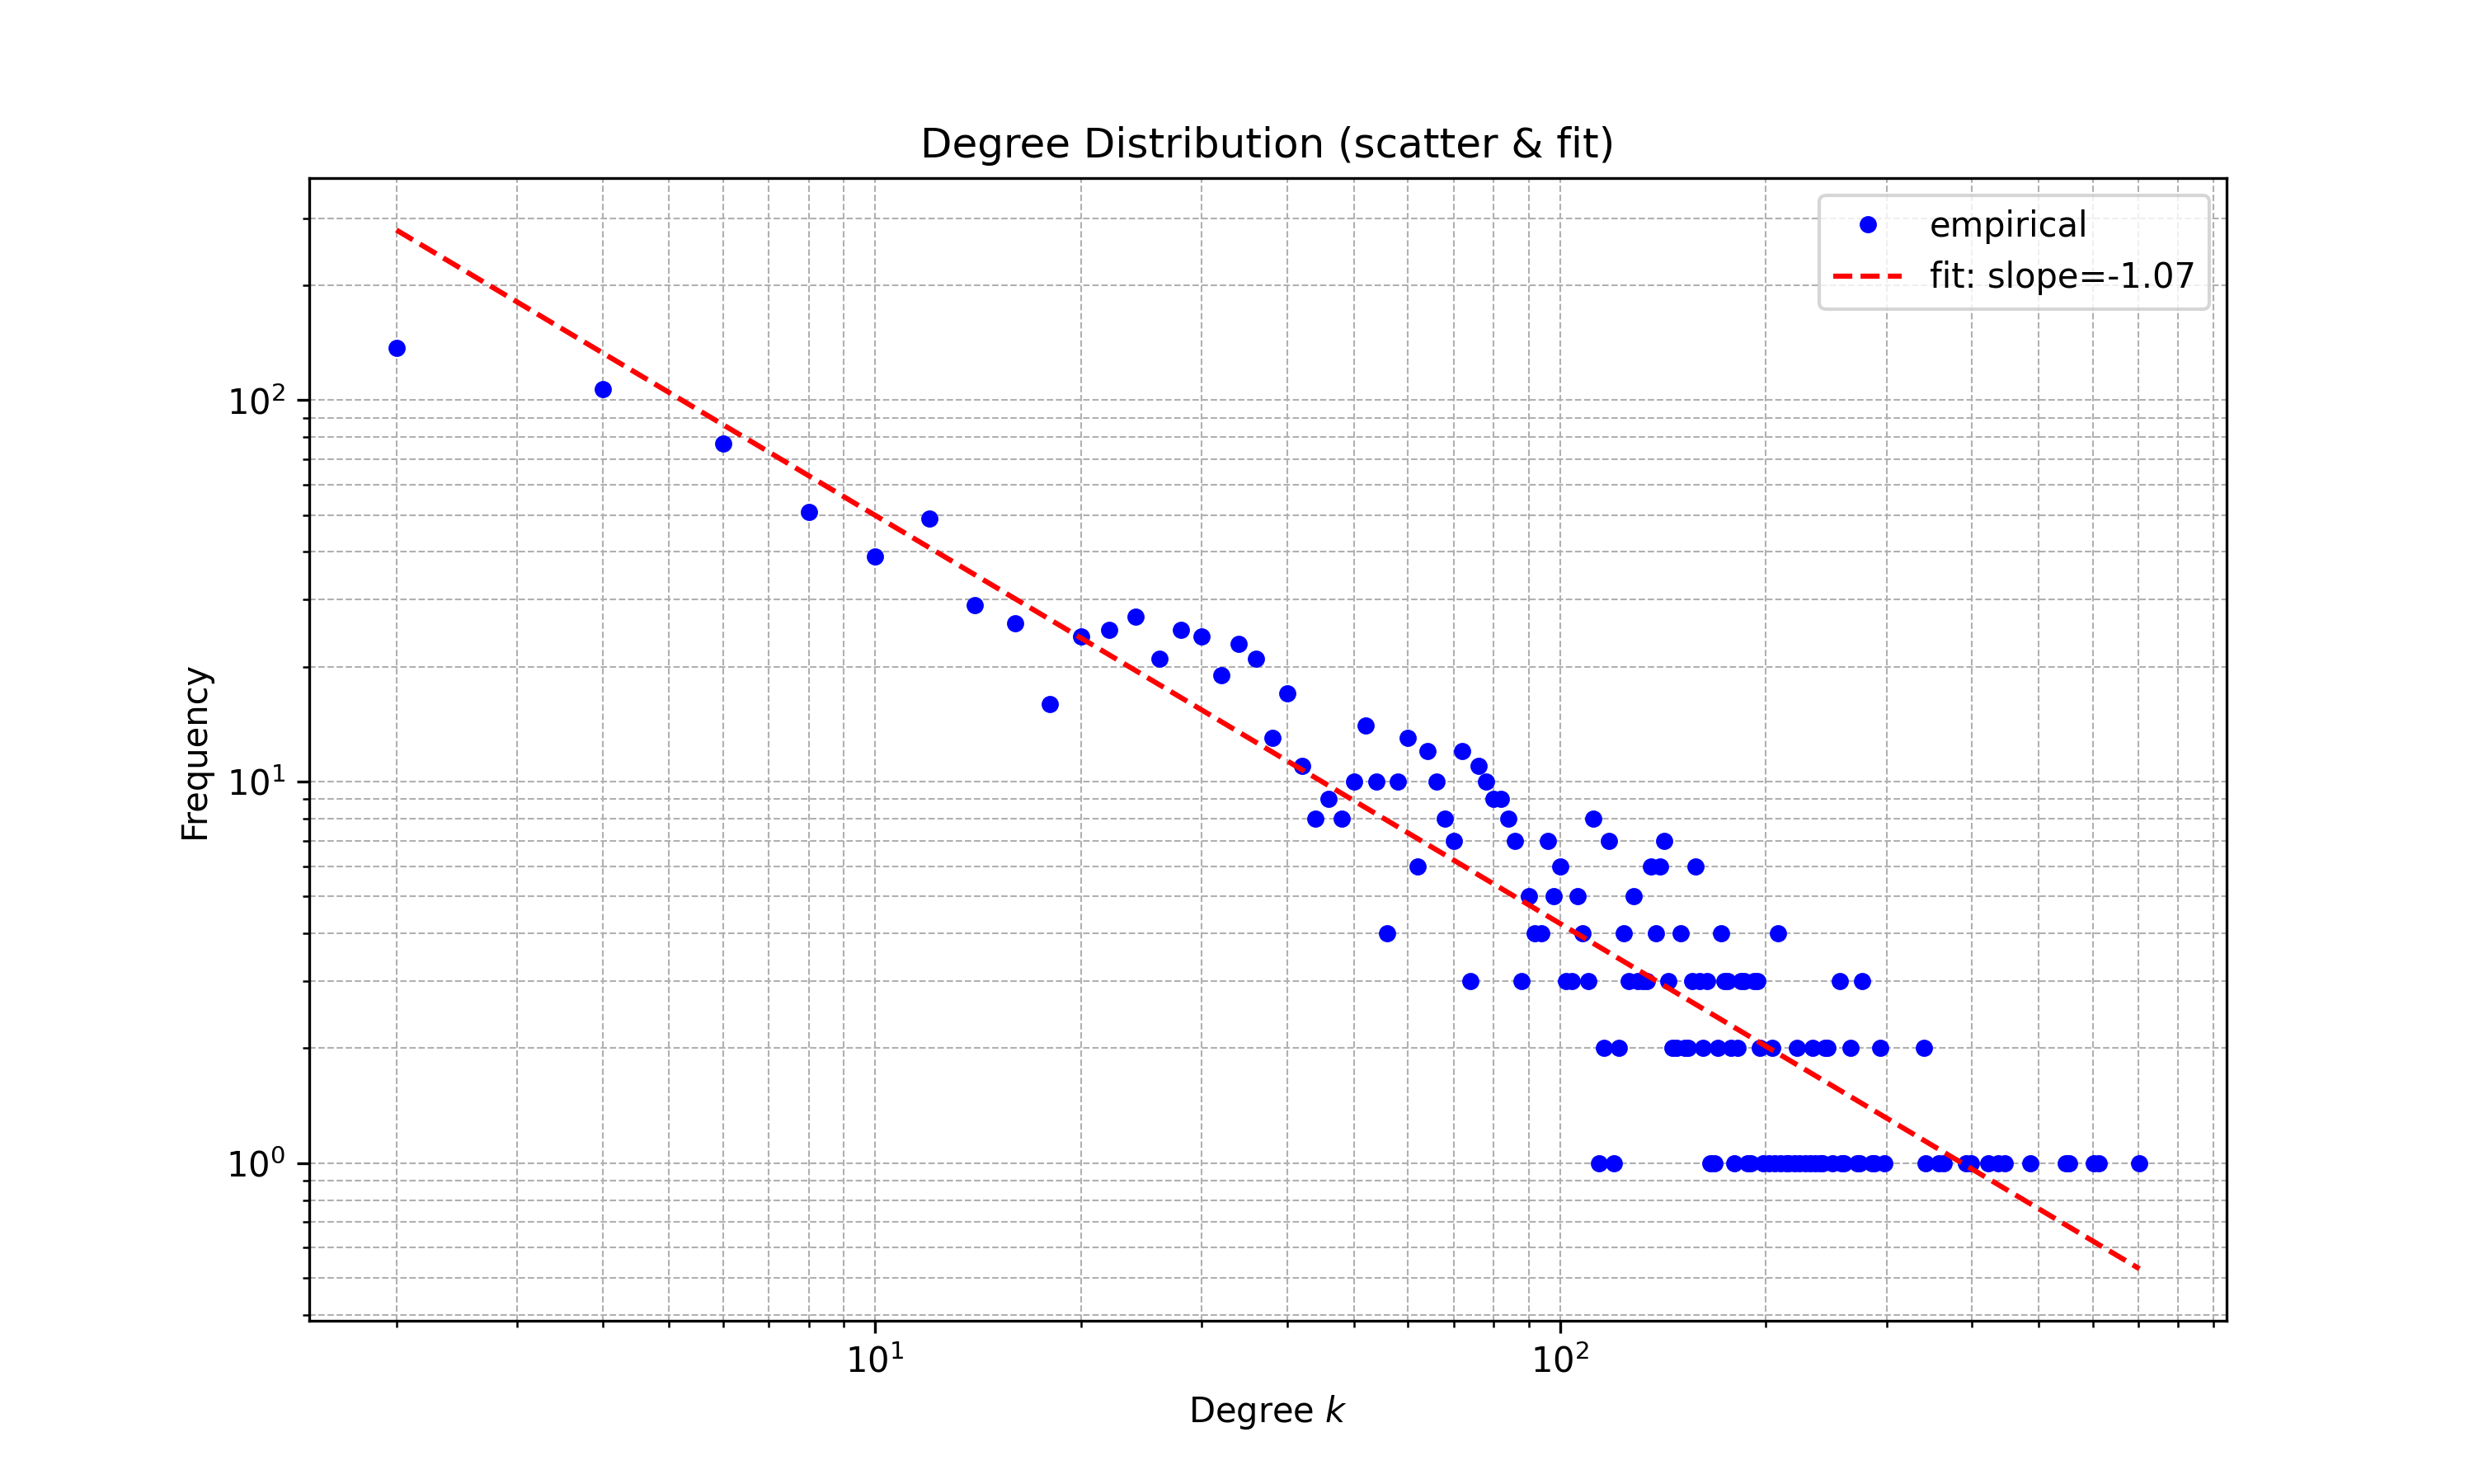
\includegraphics[width=1\textwidth]{../images/degree_scatter_fit.png}
  \caption{\label{fig:degree-scatter-fit}Raw degree counts with a power-law fit on log log axes.}
\end{figure}
This plot is shown with a red dashed line indicating a linear fit in log log space, confirming the information obtained from the previous plots and values.

Finally, the last following figure presents a spring-layout drawing of the entire network. 
\begin{figure}[H]
  \centering
  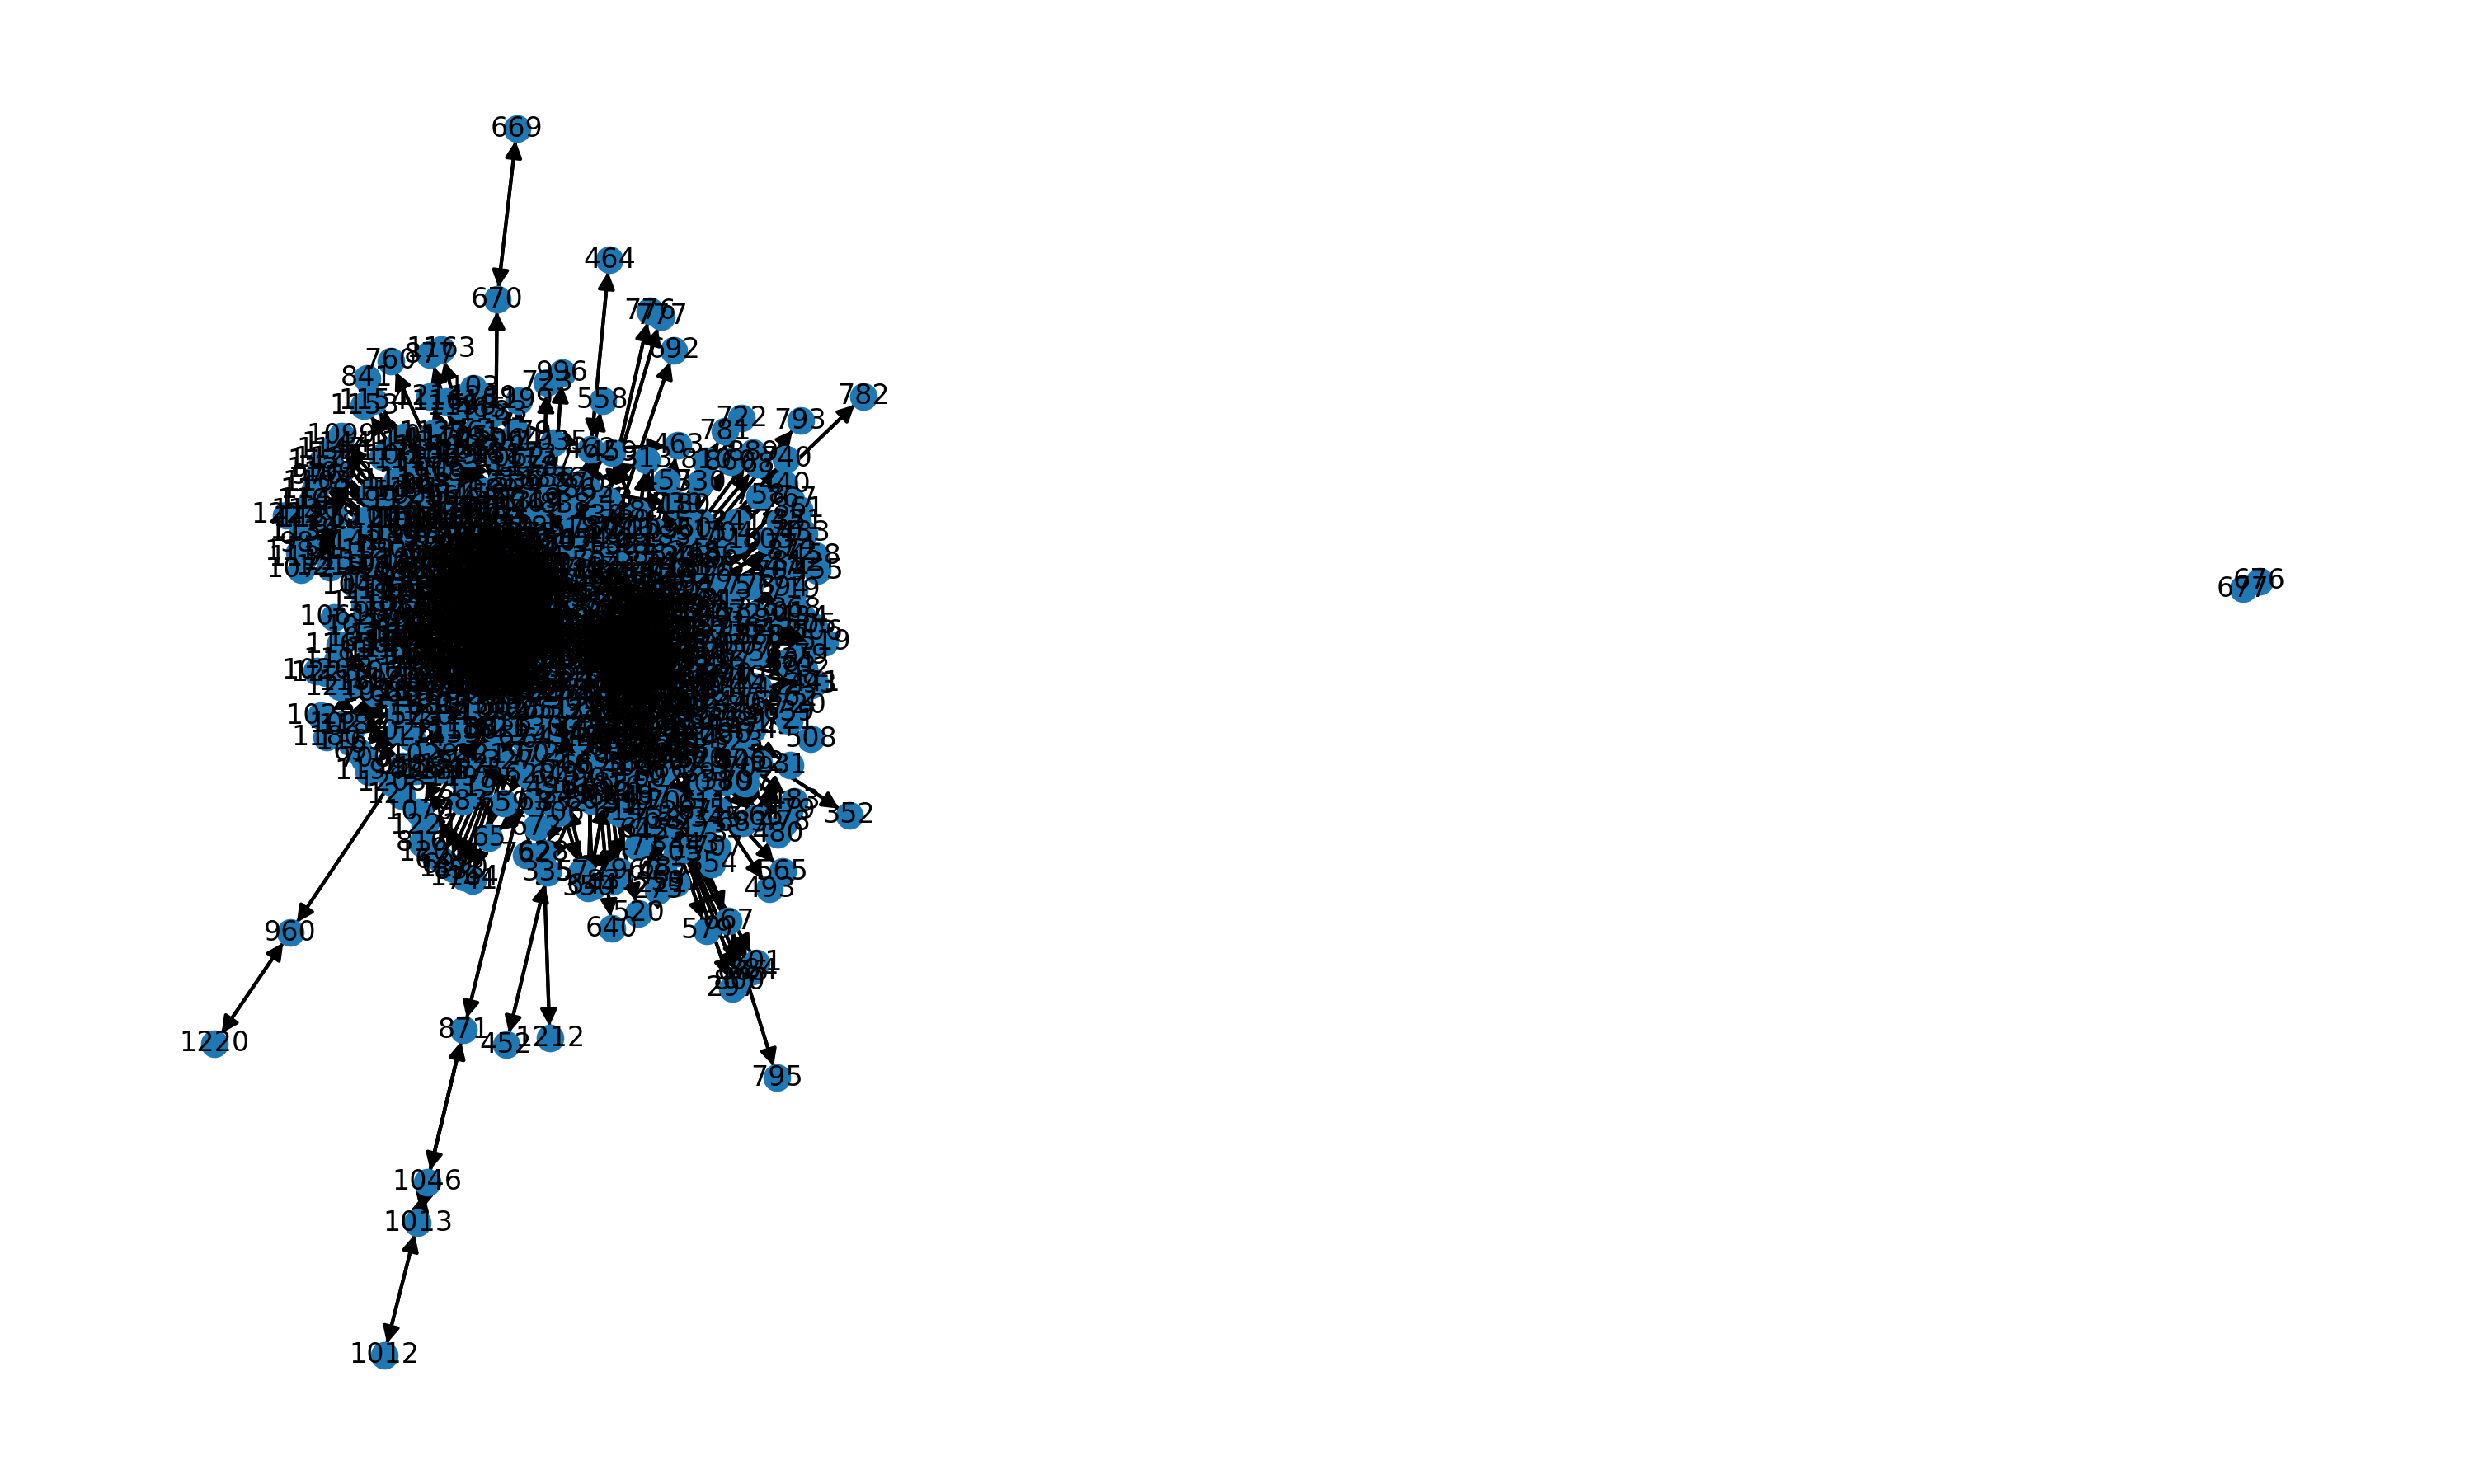
\includegraphics[width=1\textwidth]{../images/polblogs_graph.png}
  \caption{Spring-layout visualization of the full political-blogs network.}
  \label{fig:polblogs-graph}
\end{figure}
This qualitative view helps reveal community “clumps” and hub nodes in the topology of the political blogs network. Indeed, the graph drawn by itself is not very informative, due to its "blob" shape. Only $2$ nodes are outside the main blob, as we have seen in the previous sections, forming a small connected component of size $2$.

\subsection{Top 5 Central Nodes}
\label{sec:top5centrality}
Lastly, I computed three standard centrality measures, i.e.\ betweenness, closeness, and degree, on the chosen graph. The following table lists the top five nodes for each metric.

\begin{table}[H]
  \centering
  \caption{Top 5 nodes by centrality measure}
  \label{tab:top5-centrality}
  \begin{tabular}{r l l l}
    \toprule
    \textbf{Rank} & \textbf{Betweenness} & \textbf{Closeness} & \textbf{Degree} \\
    \midrule
    1 & Node~460: 0.0977 & Node~163: 0.5185 & Node~~~ 9:   0.5740 \\
    2 & Node ~~~9: 0.0881 & Node~~~ 9: 0.5178 & Node~163: 0.5004 \\
    3 & Node~229: 0.0680 & Node~~ 21: 0.5023 & Node~460: 0.4922 \\
    4 & Node~163: 0.0494 & Node~~~ 5: 0.4976 & Node~~~ 5: 0.4530 \\
    5 & Node~~ 21: 0.0475 & Node~312: 0.4937 & Node~~ 21: 0.4481 \\
    \bottomrule
  \end{tabular}
\end{table}

It is obvious that there are 3 recurring nodes inside the table: 
\begin{itemize}
  \item node \textbf{460}
  \item node \textbf{163}
  \item node \textbf{9}
\end{itemize}

Node 460 leads in betweenness centrality, indicating it sits on many shortest paths and serves as a critical bridge in the network. Nodes 163 and 9 rank highest in closeness, meaning they have the shortest average distance to all other blogs and are thus highly accessible. Finally, degree centrality highlights node 9 as the most connected (with 57.4\% of possible links), followed by nodes 163 and 460. The most interesting thing to note is that the strong overlap among these top nodes underscores a small set of influential blogs that likely dominate information flow and connectivity in the network.

\vspace{0.5cm}

In the following sections, I will further analyze the structure of this graph, in order to reveal what informations lie hidden in its clump structure. In particular, I will use three different algorithms, i.e.\ Girvan-Newman, Louvain, and Leiden. 


\section{Part 2: Community analysis}\label{sec:part2}
In this section, I will investigate the community structure of the political blogs graph using three different algorithms: Girvan-Newman, Louvain, and Leiden. I will also measure the execution time of each algorithm, in order to compare their performance.

\subsection{Girvan-Newman algorithm}
I first executed the Girvan-Newman (GN) hierarchical algorithm and tracked modularity as we split the network progressively. The following table summarizes the result.

\begin{table}[H]
  \centering
  \caption{Girvan-Newman modularity at successive splits}
  \label{tab:gn-modularity}
  \begin{tabular}{r c c}
    \toprule
    \textbf{Level} & \textbf{\# Communities} & \textbf{Modularity} \\
    \midrule
     1  &  3  & 0.0006 \\
     2  &  4  & 0.0007 \\
     3  &  5  & 0.0008 \\
     4  &  6  & 0.0010 \\
     5  &  7  & 0.0018 \\
     6  &  8  & 0.0019 \\
     7  &  9  & 0.0020 \\
     8  & 10  & 0.0021 \\
     9  & 11  & 0.0023 \\
    10  & 12  & 0.0024 \\
    11  & 13  & 0.0024 \\
    \bottomrule
  \end{tabular}
\end{table}

The highest modularity, $Q = 0.0024$, occurs at the 10th split (leven 10, 12 communities). 
Although the absolute modularity values are low—reflecting the relatively weak community structure in this dataset—the monotonic rise up to 12 communities suggests that finer partitions better capture the latent grouping of political blogs, showing better cohesion than its random counterparts.
The Girvan-Newman algorithm was by far the worst in terms of execution time, around $20$ minutes, making it impractical for larger networks. This confirms the known $O(m^{2}n)$ complexity of the algorithm.

\begin{figure}[H]
  \centering
  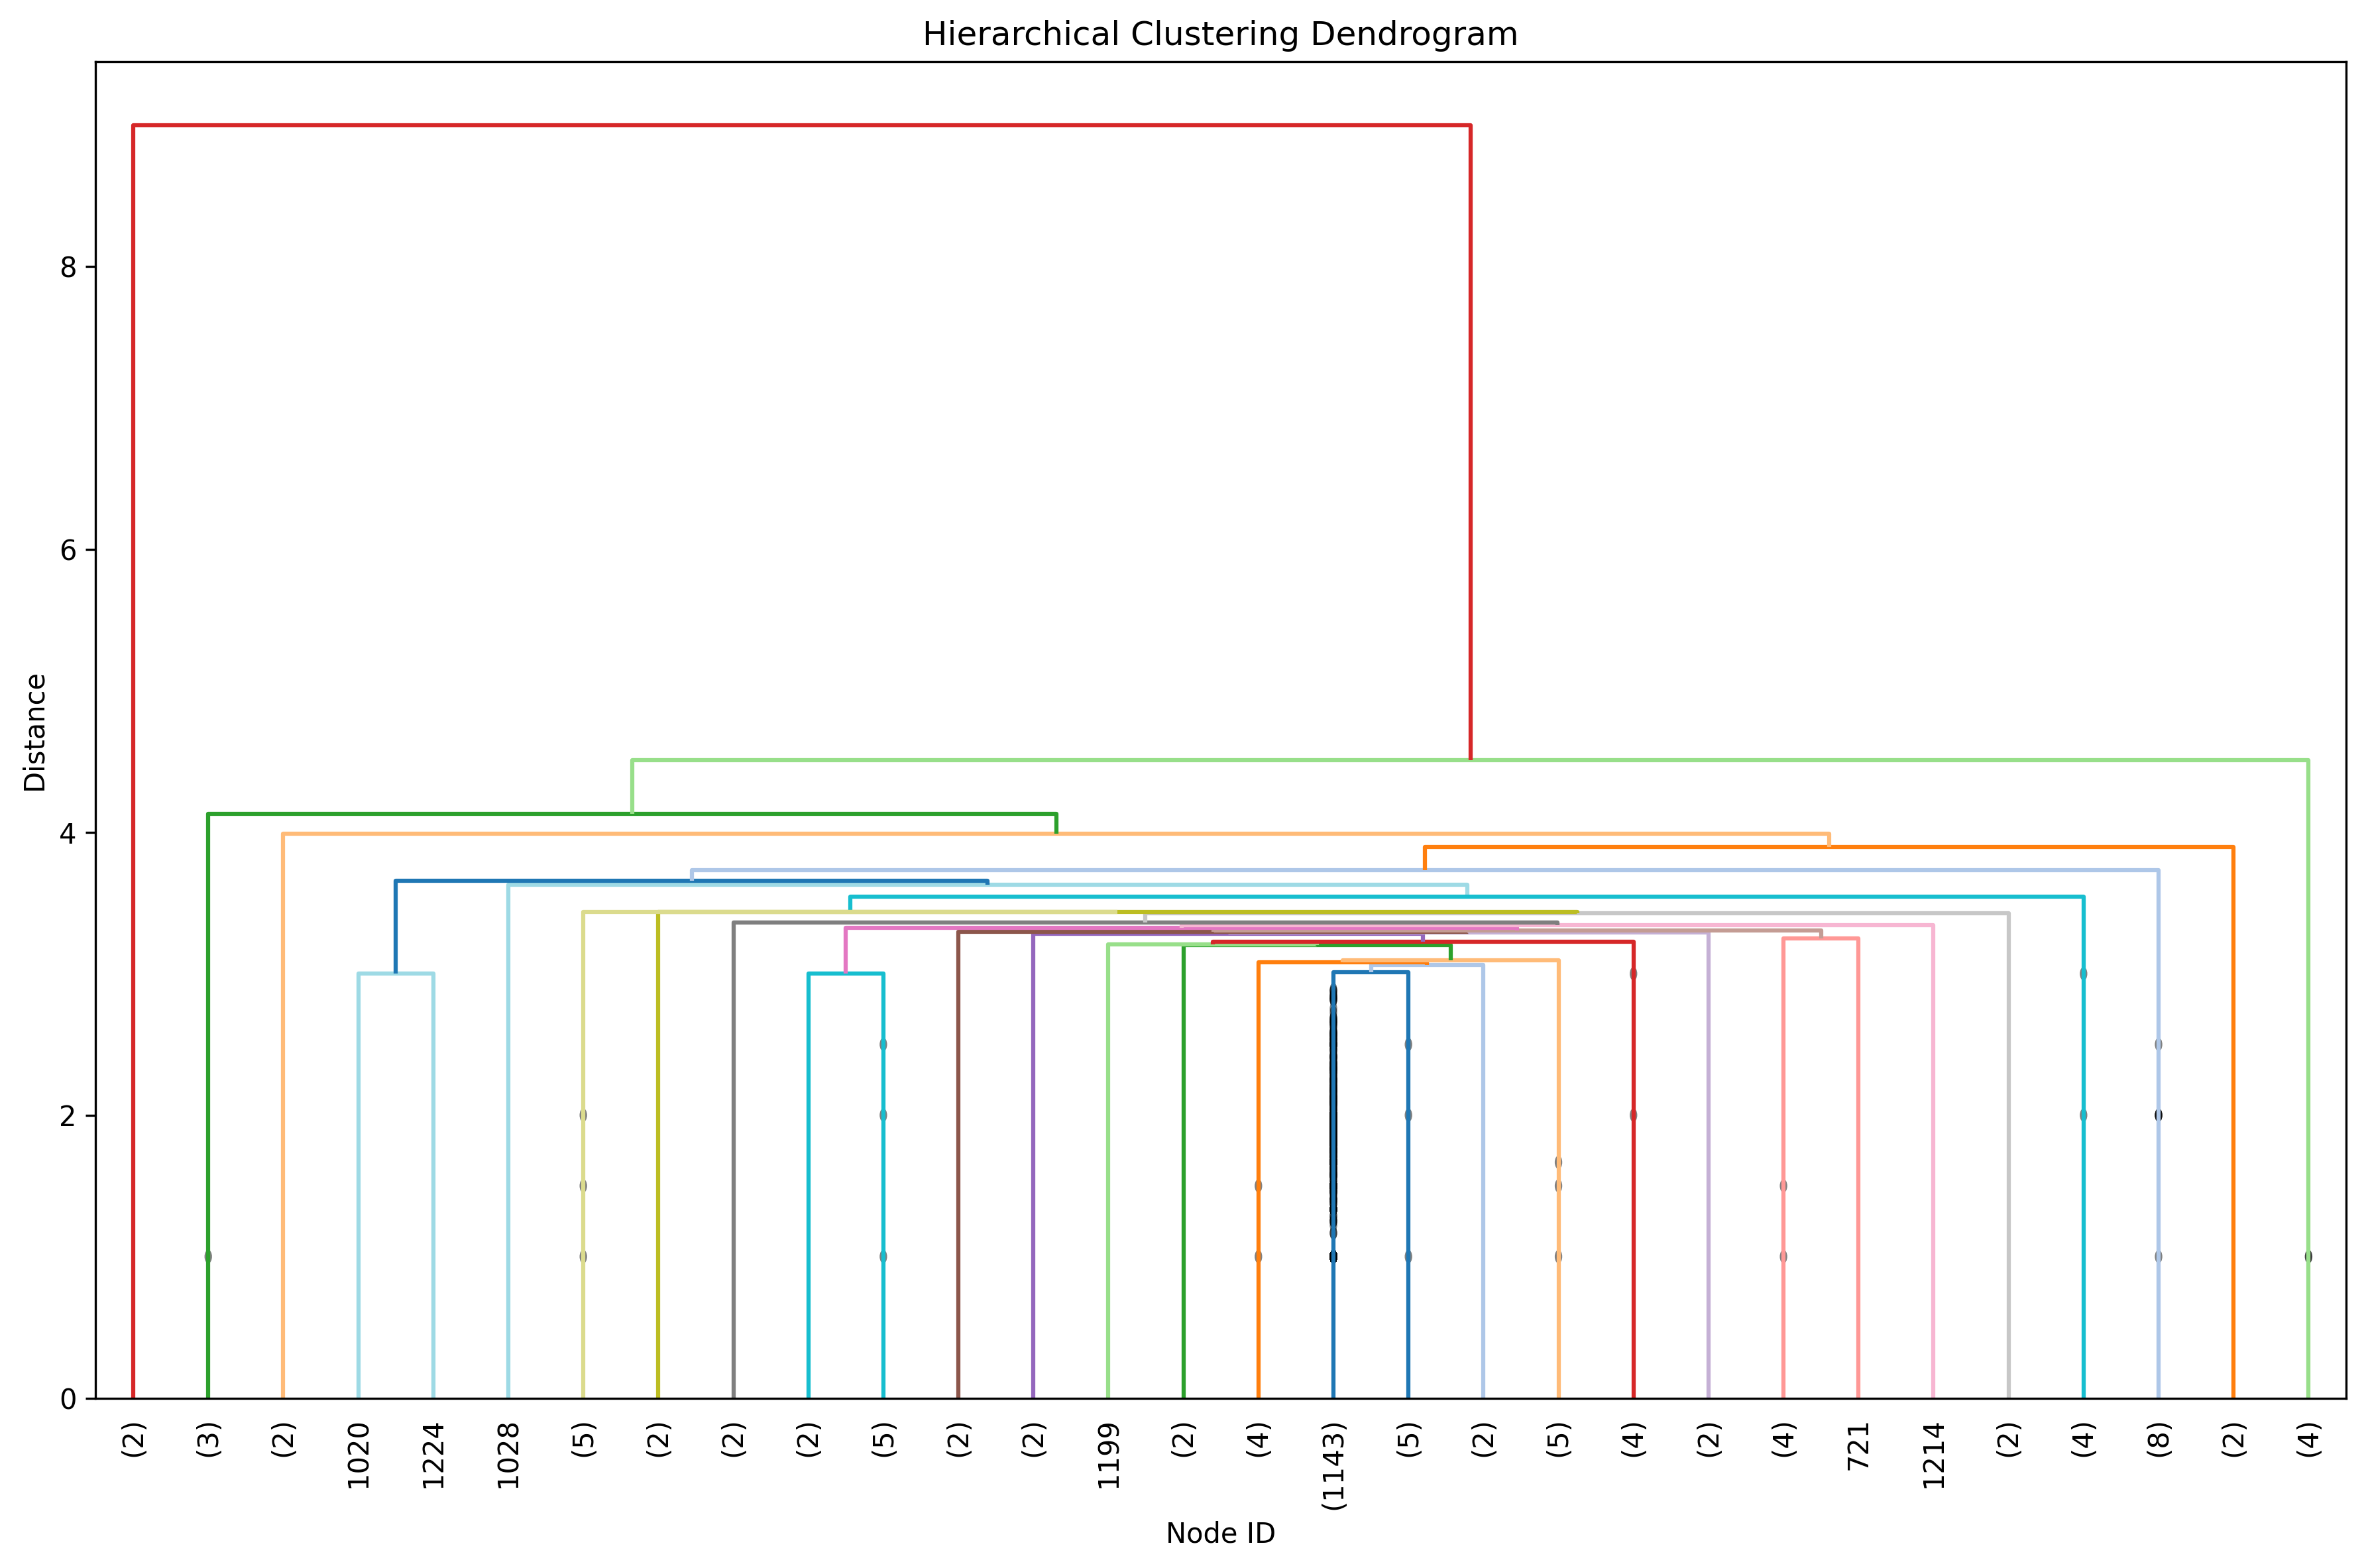
\includegraphics[width=1\textwidth]{../images/dendrogram.png}
  \caption{Girvan-Newman Dendrogram}
  \label{fig:gn-dendrogram}
\end{figure}

\begin{figure}[H]
  \centering
  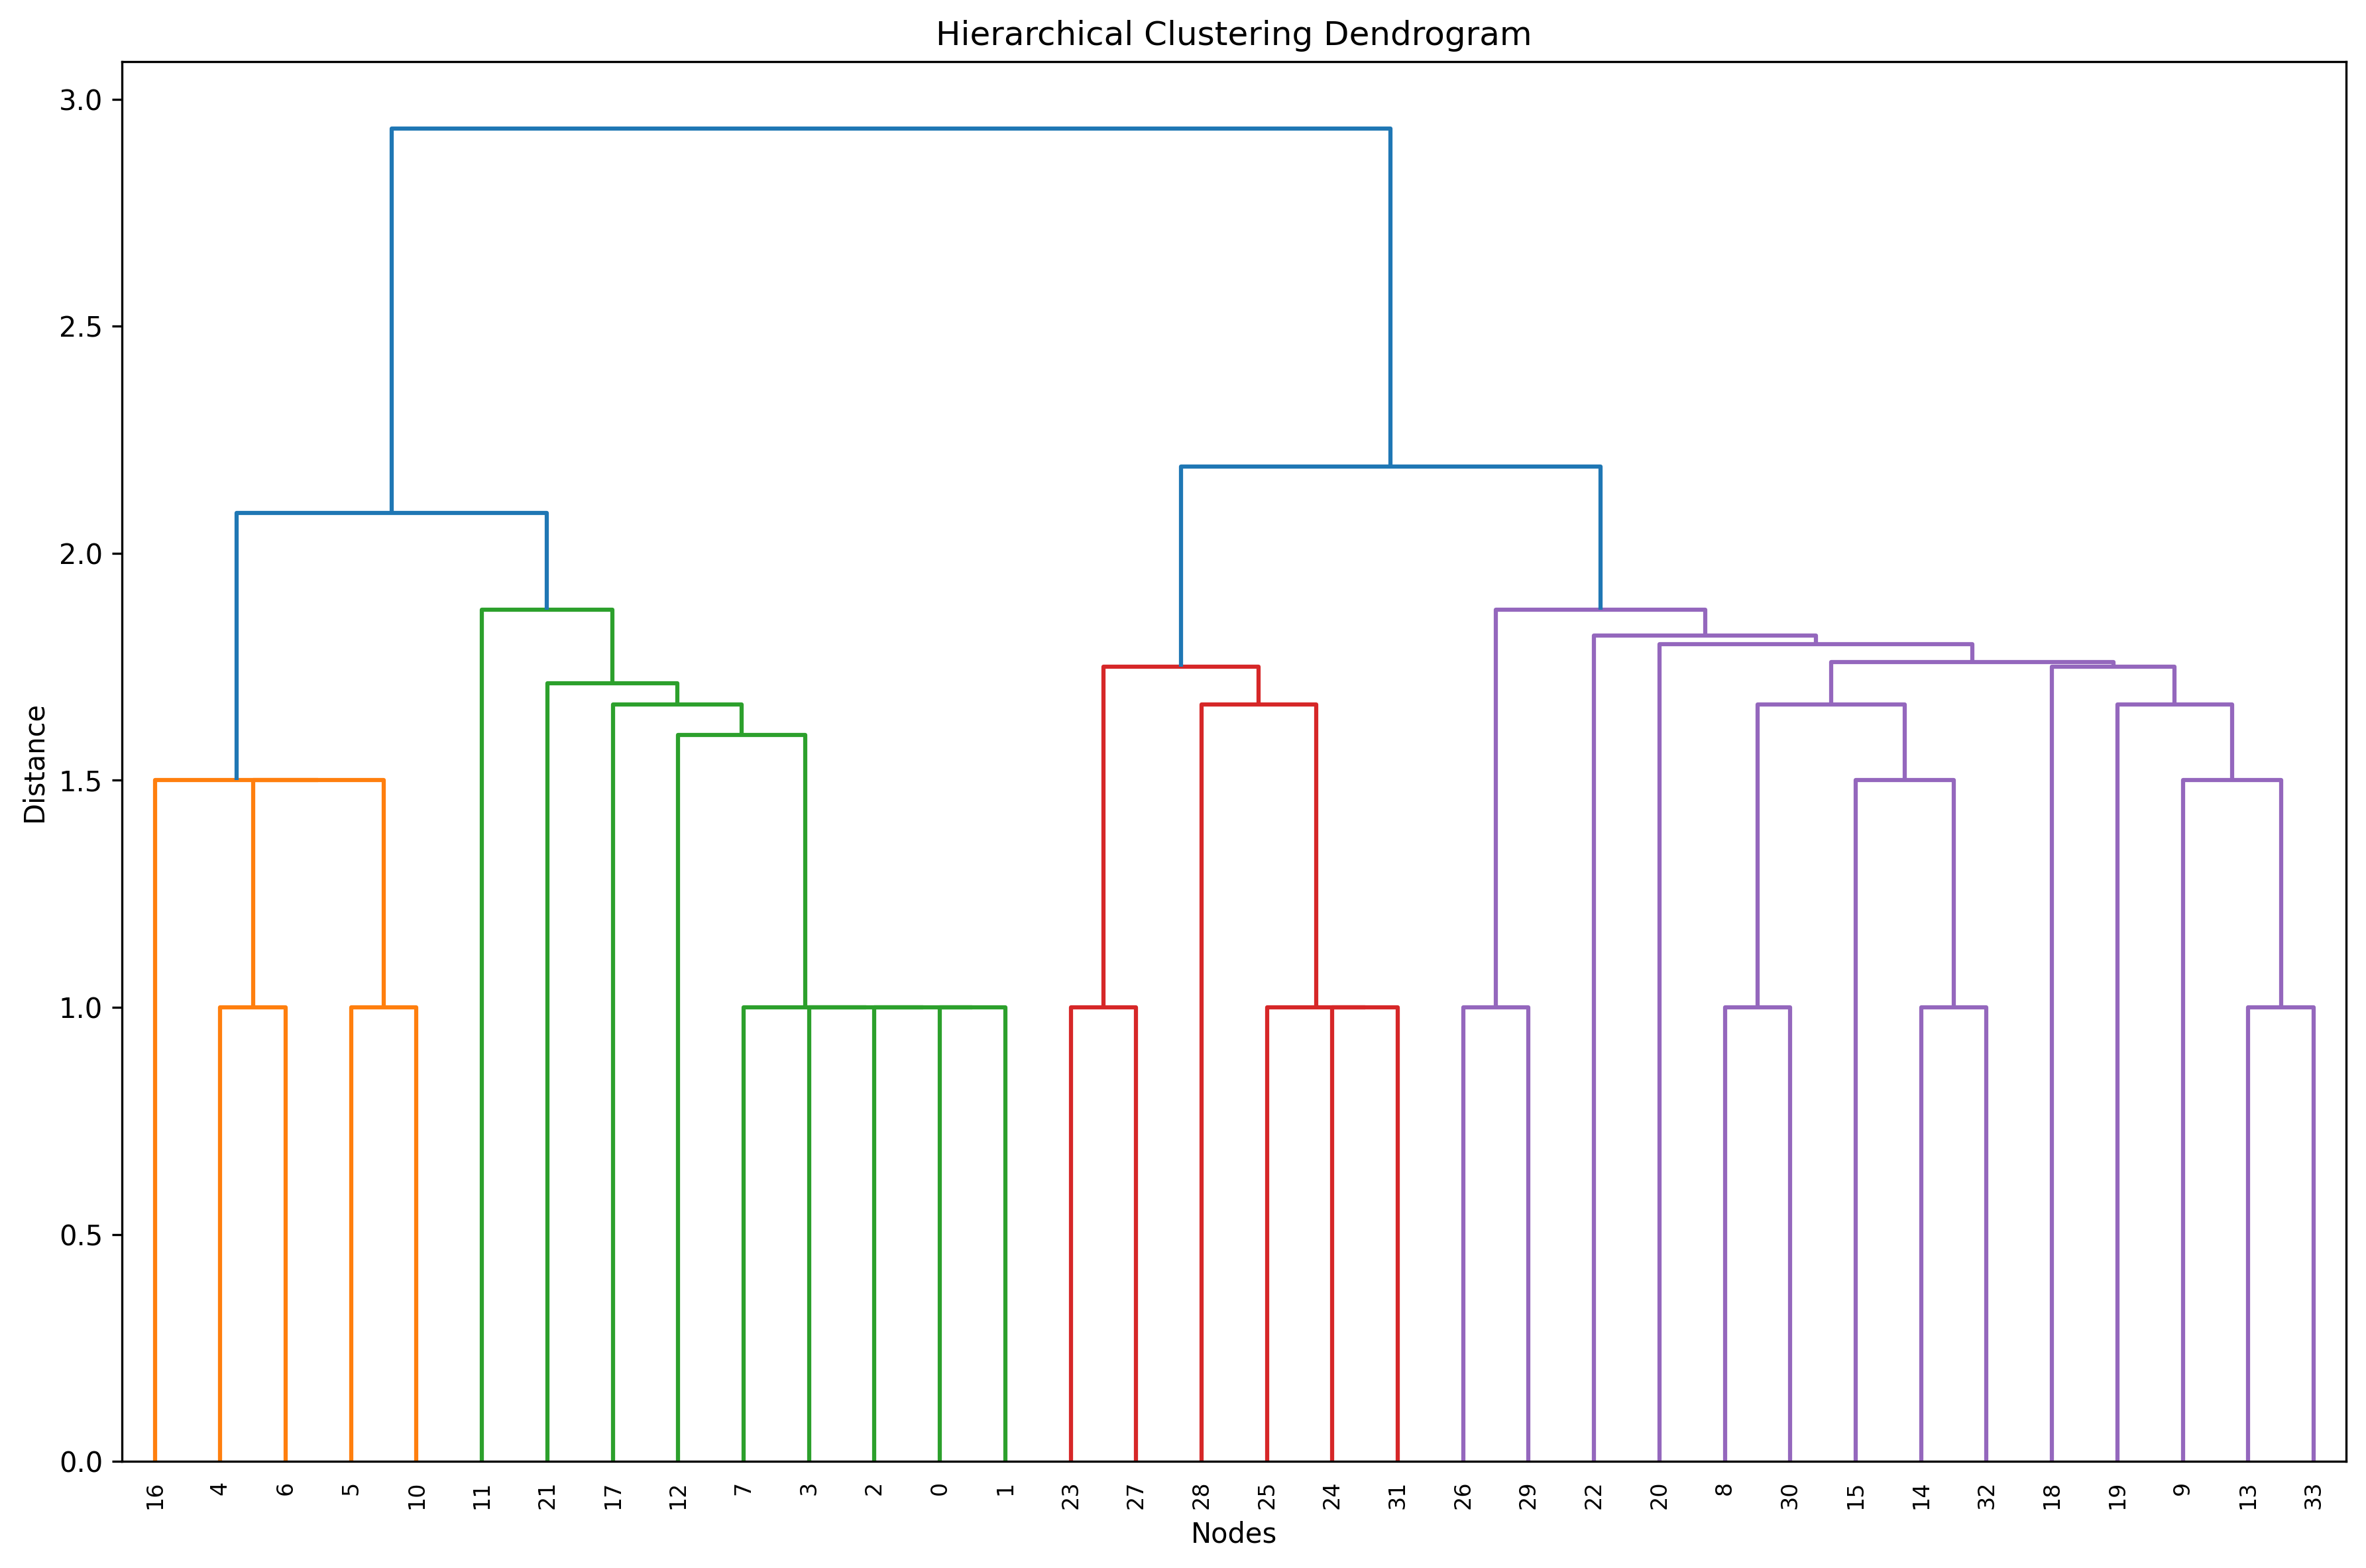
\includegraphics[width=1\textwidth]{../images/karate_club_dendrogram.png}
  \caption{Zachary's Karate Club Dendrogram, for reference}
  \label{fig:zkc-dendrogram}
\end{figure}

Figure 6 shows a truncated Girvan-Newman dendrogram for the political blogs network, showing only the last 30 agglomeration steps.  
At the bottom, each leaf is labeled by its cluster index (or, for contracted branches, by the number of merged nodes in parentheses), and contracted subtrees appear as orange triangles (with the very first split in blue).  
The vertical axis measures the linkage distance (i.e.\ the modularity-based “cost” of combining two clusters), so taller branches correspond to merges that bridge more loosely connected portions of the network.


\subsection{Louvain and Leiden algorithms}
I then executed the Louvain method with the help of a pair of python scripts from AulaWeb and refactored both  of them into the \texttt{ribba\_louvain()} and \texttt{ribba\_leiden()} functions.
Equally to the Girvan-Newman algorithm, the Louvain algorithm found $12$ communities in the political blogs network, completing in $1.7$ seconds, thanks to its optimized nature.
The different number of communities found by the Louvain method compared to Girvan-Newman is not surprising, as the two algorithms employ different approaches to community detection.
The Louvain method uses a greedy optimization strategy to maximize modularity, while Girvan-Newman relies on edge removal to iteratively reveal community structure.

Indeed, the Louvain algorithm found modularity $Q = 0.4271$, which is higher than the maximum modularity found by Girvan-Newman, indicating that the Louvain method is more effective at identifying cohesive communities in this dataset.

Additionally, also the Leiden method, found the same number of communities as Girvan-Newman, i.e.\ $12$, but in order of magnitudes faster (less than half a second), as expected, since it is a refinement of the Louvain method (Leiden uses a local optimization approach to improve the community structure found by Louvain).

Finally, the Leiden method achieved a modularity of $Q = 0.427$, which is practically the same as the modularity of the Louvain method, indicating that both algorithms are effective at identifying cohesive communities in this dataset, but Leiden is a little bit faster than Louvain, as expected (even though the speedup is also due the different libraries).



\subsubsection{Performance Comparison}
The following table summarizes the execution times and relative speedups compared to the Girvan-Newman baseline. Notably, Louvain achieves a $636$ $\times$ speedup, while Leiden attains a $2625$ $\times$ speedup over Girvan-Newman and is $4.13$ $\times$ faster than Louvain.

\begin{table}[H]
  \centering
  \begin{tabular}{lrr}
    \toprule
    \textbf{Algorithm}     & \textbf{Time (s)} & \textbf{Speedup vs GN} \\
    \midrule
    Girvan-Newman          & $1061.14$     & $1\times$              \\
    Louvain                &   $1.76$      & $636\times$    \\
    Leiden                 &   $0.43$      & $2625\times$   \\
    \midrule
    Leiden \textbf{vs} Louvain      &                   & $4.13\times$      \\
    \bottomrule
  \end{tabular}
  \caption{Execution times and speedups for community detection methods in Part 2.}
  \label{tab:part2_times}
\end{table}



\vspace{0.5cm}
As expected, the Louvain and Leiden algorithms run much faster than the Girvan-Newman algorithm.
The Girvan-Newman algorithm yields a very low modularity on the real political blogs network, indicating that its stepwise edge-removal procedure fails to uncover cohesive communities in this dataset.
In contrast, Louvain and Leiden obtain a higher modularity, indicating that they are more effective at identifying communities in this network, demonstrating their strength at rapidly identifying dense intra-community connections that the Girvan-Newman method often misses.

Considering the scale of network taken into consideration (roughly 1\,200 nodes and 33\,000 edges), the enormous speed and quality advantage of Louvain and Leiden makes them the obvious choice for practical community detection, even though Louvain was only around a second slower than Leiden, but that is probably due to Leiden being implemented in \texttt{igraph} and not in \texttt{NetworkX}; still the Louvain method found $11$ communities, while Leiden found $12$.

In the next section I will also visualize and evaluate the resulting graphs, considering the partitions produced by every algorithm.


\section{Part 3: Evaluation of the Quality of the Communities}\label{sec:part3}
Even in the absence of a known “ground truth,” it is possible to assess how consistently different algorithms partition the same network by using pairwise similarity metrics. Normalized Mutual Information (NMI) and the Adjusted Rand Index (ARI) both quantify the agreement between two community assignments—higher values indicate that the two algorithms group nodes in a similar way. Importantly, NMI remains meaningful even when the algorithms produce different numbers of communities.

The following table shows the pairwise NMI and ARI scores. These metrics do not tell us which partition is “correct,” only how much two algorithms agree, and how similar their partitions are.

\begin{table}[H]
  \centering
  \caption{Pairwise NMI and ARI between community assignments}
  \label{tab:partition-similarity}
  \begin{tabular}{l c c}
    \toprule
    \textbf{Comparison}                 & \textbf{NMI}  & \textbf{ARI}  \\
    \midrule
    Girvan-Newman vs Louvain            & 0.2036        & 0.0638        \\
    Girvan-Newman vs Leiden             & 0.2008        & 0.0632        \\
    Louvain vs Leiden                   & 0.9855        & 0.9926        \\
    \bottomrule
  \end{tabular}
\end{table}

Each of the three algorithms found 12 communities, but their partitions differ substantially. 
Girvan-Newman has low agreement with both Louvain and Leiden 
(\(\mathrm{NMI}\approx0.2036\), \(\mathrm{ARI}\approx0.0638\)), indicating that its hierarchical edge-removal process yields a grouping largely inconsistent with modularity-based methods. 
By contrast, Louvain and Leiden agree almost perfectly 
(\(\mathrm{NMI}\approx0.9855\), \(\mathrm{ARI}\approx0.9926\)), reflecting Leiden's role as a refinement of Louvain, even though the small difference in execution time is probably due to the fact that Leiden is implemented in \texttt{igraph} and not in \texttt{NetworkX}.

In the end, the Girvan-Newman algorithm fails to capture the community structure of the political blogs network (as shown in Figure 8), while both Louvain and Leiden produce high-quality partitions that are nearly identical and, in practice, interchangeable, with Leiden returning a marginally higher modularity.



\section{Part 4: Visualization of the communities}\label{sec:part4}
\newcommand{\FigGNVis}{../images/gn_communities.png}
\newcommand{\FigLouvainVis}{../images/louvain_communities.png}
\newcommand{\FigLeidenVis}{../images/leiden_communities.png}

In this section, I will show the graphical renderings of the communities found during this first assignment on the political-blogs network. 
Each node is colored according to its community label, in order to get a better visual comparison of how the different algorithms partition the network. 

\begin{figure}[H]
  \centering
  \includegraphics[width=1\textwidth]{\FigGNVis}
  \caption{Girvan-Newman communities}
  \label{fig:gn-visualization}
\end{figure}

\begin{figure}[H]
  \centering
  \includegraphics[width=1\textwidth]{\FigLouvainVis}
  \caption{Louvain communities}
  \label{fig:louvain-visualization}
\end{figure}

\begin{figure}[H]
  \centering
  \includegraphics[width=1\textwidth]{\FigLeidenVis}
  \caption{Leiden communities}
  \label{fig:leiden-visualization}
\end{figure}


The Girvan-Newman partition in Figure 8 shows one overwhelmingly large community (blue) containing nearly all nodes, with the other eleven communities reduced to tiny peripheral fragments. 
This pattern indicates that the successive edge removals of Girvan-Newman isolate only a few small subgraphs and otherwise leave one monolithic cluster, failing to localize the underlying communities.

By contrast, the Louvain result in Figure 9 splits the network into two major cohesive blocks (teal and light blue) alongside several medium, and small sized communities. 
Due to its greedy modularity maximization, it merges densely connected regions into broader groups, yielding a more balanced hierarchy of community sizes, and reflecting the real world bipolarization of the political blogs around the 2004 presidential elections.

Finally, the Leiden partition shown in Figure 10 also produces twelve communities but with tighter intra community cohesion and fewer near isolated nodes. 
As a refinement of Louvain, Leiden corrects poorly connected subdivisions, resulting in more evenly sized clusters and clearer boundary delineation.

In the end, the Girvan-Newman algorithm tends to isolate a single giant component and many trivial splits, while both Louvain and Leiden capture a more compliance situation, in a typical political fashion.


\section{Conclusions}\label{sec:conclusions}
Even though the graph initially appeared to be a complex and tangled blob-shape, I was still able to analyze its properties and communities, thanks to the use of the \texttt{NetworkX} and \texttt{igraph} python libraries.
In particular, the final graphs about the inner communities inside the \texttt{polblogs} graph showed a clear bipolarization of the nodes with 2 dominant partitions, obviously for the 2 candidates more likely to win the presidential election of that time, surrounded by smaller groups and a pair of blogs connected with one another, but disconnected from the dominant graph.

In conclusion, while Girvan-Newman produced only trivial fragments alongside one giant cluster (low modularity), Louvain and Leiden delivered high-quality partitions (modularity \(\approx0.43\)) in an average of a second, and agreed nearly perfectly (NMI=0.956, ARI=0.979). 
The Leiden refinement in particular yielded well-connected, evenly sized communities with minimal isolated nodes.


\appendix
\section{Code Output}\label{sec:appendix-output}
The output of the code used to compute the graph properties is both attached in the assignment archive as a text file and included here \attachfile{../results.txt} for reference. 

% \lstinputlisting{../res}



\end{document}